\documentclass{zbc-report}

\usetikzlibrary{shapes.geometric}  % Including shapes.geometric for TikZ
\usepackage[normalem]{ulem}
\useunder{\uline}{\ul}{}

%% Set up the bibliography
\usepackage[backend=biber, style=apa]{biblatex}
\addbibresource{main.bib}

%% Additional packages and commands
\usepackage{parskip}
\setlist{itemsep=-2pt} % Reducing white space in lists slightly
\renewcommand{\deg}{\si{\degree}\xspace} % Use \deg easily, everywhere

%% Set up the graphics path
\usepackage{tikz}
\usetikzlibrary{angles, quotes, shapes.geometric, arrows.meta, positioning}
\tikzstyle{block} = [rectangle, rounded corners, minimum width=3cm, minimum height=1cm,text centered, draw=black, fill=blue!10]
\tikzstyle{arrow} = [thick, ->, >=Stealth]

%% Set up the minted package
\usepackage[cachedir=_minted]{minted}
\setminted{
    linenos=true,
    breaklines=true,
    fontsize=\footnotesize,
    frame=lines,
    framesep=2mm,
    baselinestretch=1.2,
    bgcolor=gray!10,
    style=vs,
    mathescape=true,
}

%% ----------------------------------------------------------------------
%%    Begin of document + Frontmatter (Roman page numbering)
%% ----------------------------------------------------------------------

\begin{document}

\frontmatter

%% Define the main parameters
\title{Synopsis}
\subtitle{AI and Machine Learning \\ 4. Semester}
\author{Carsten Lydeking}

\subject{Book recommender using NLP} % Cover only
\large\affiliation{Zealand Academy of Technology and Business} % Cover only
\coverimage{figures/template-figures/binary.jpg} % Aspect ratio of 2:3 (portrait) recommended
\definecolor{title}{HTML}{4884d6} % Color for cover title

\makecover

\begin{titlepage}

\begin{center}

%% Print the title
{\makeatletter
\largetitlestyle\fontsize{45}{45}\selectfont\@title
\makeatother}

%% Print the subtitle
{\makeatletter
\ifdefvoid{\@subtitle}{}{\bigskip\titlestyle\fontsize{20}{20}\selectfont\@subtitle}
\makeatother}

\bigskip
\bigskip

%% Print the name of the author
{\makeatletter
\largetitlestyle\fontsize{25}{25}\selectfont\@author
\makeatother}

\bigskip
\bigskip

%% Print table with names and student numbers
\setlength\extrarowheight{2pt}
\begin{tabular}{c}
    cal002@edu.zealand.dk \\
\end{tabular}

\vfill

%% Print some more information at the bottom
\begin{tabular}{l r}
    Lecturer, AI and ML:   & Jens Peter Andersen \\
    Project Deadline: & \ddmmyydate{28/05/2025} \\
    Handed-in:       & \ddmmyydate{\today} \\
    Semester:        & 4. Semester\\
    Word Count:      & 23.460 Characters (including spaces) \\ %% Counted using texcount, not included in template
\end{tabular}

\bigskip
%% Add a source and description for the cover and optional attribution for the template
\begin{tabular}{l r}
    Cover: & Generated image of binary using DALL-E \\
    Style: & ZBC template -- created by Carsten Lydeking (Cally) \\
\end{tabular}


%% Insert the Zealand logo at the bottom of the page
\begin{tikzpicture}[remember picture]
    \node[above=10mm] at (current page.south) {%
        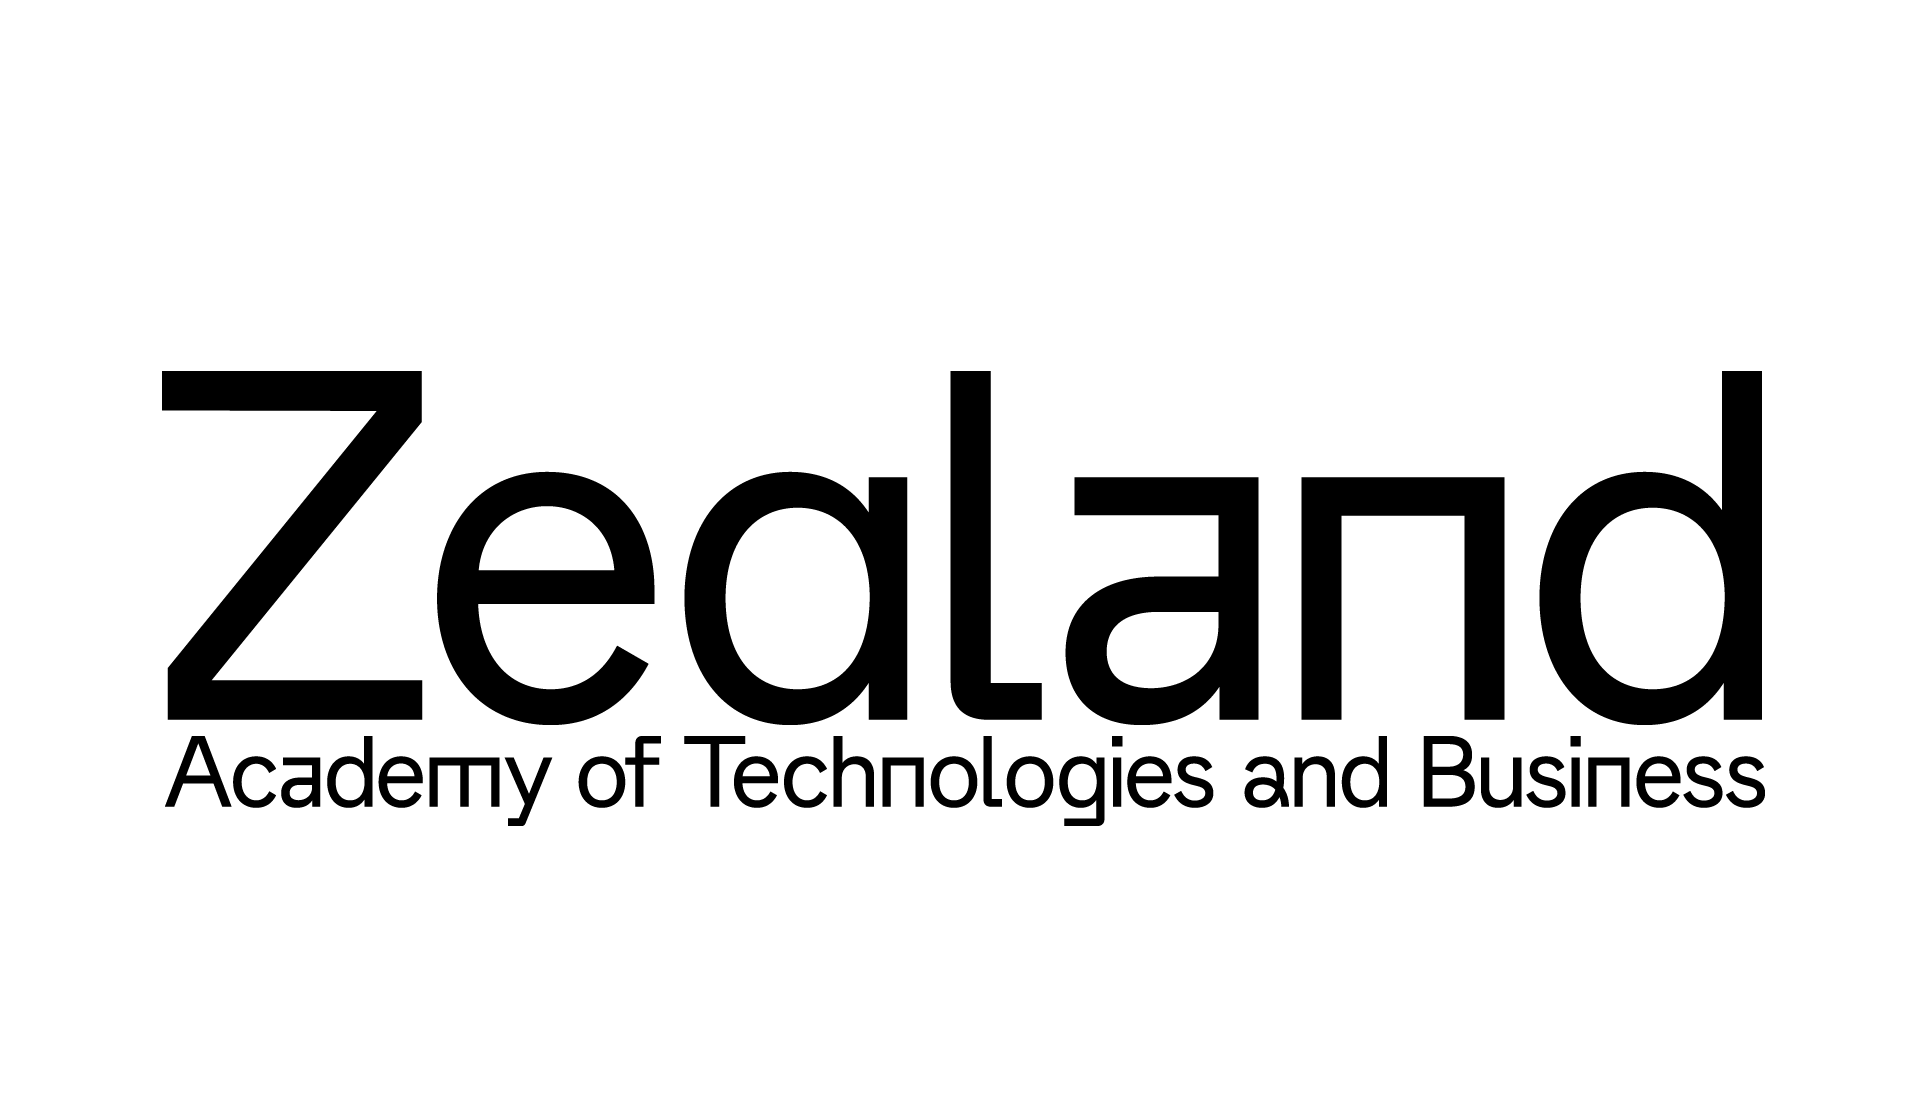
\includegraphics[width=0.35\textwidth]{figures/template-figures/zealandcombinedlogo}
    };
\end{tikzpicture}

\end{center}

\end{titlepage}

\tableofcontents
%\listoffigures
%\listoftables

%\chapter*{Nomenclature}
\addcontentsline{toc}{chapter}{Nomenclature}

\section{Abbreviations and definitions}
\label{sec:abbreviations}
The following abbreviations and definitions are used throughout the report:

\renewcommand{\arraystretch}{2}
\begin{longtable}{l p{13.5cm}}
    \textbf{Abb.}  & \textbf{Definition}  \\ \hline
        DB           & Database: A structured collection of data stored electronically. \\ \hline
        RDB          & Relational Database: A type of DB that stores and provides access to data points that are related to one another. \\ \hline
        DBMS         & Database Management System: Software that handles the storage, retrieval, and updating of data in a database. \\ \hline
        RDBMS        & Relational DBMS: A database management system based on the relational model introduced by E.F. Codd. \\ \hline
        SQL          & Structured Query Language: A programming language used to manage and manipulate relational databases. \\ \hline
        CRUD         & Create, Read, Update, Delete The four basic operations of persistent storage: adding, retrieving, modifying, and removing data. \\ \hline
        GUI          & Graphical User Interface  A user interface that allows users to interact with electronic devices using graphical icons and visual indicators. \\ \hline
        PK           & Primary Key:A unique identifier for each record in a database table. \\ \hline
        FK           & Foreign Key: A field in a database table that links to the primary key of another table. \\ \hline
        NML          & Normalization: In relation to RDB design, the process of organizing the columns (attributes) and tables (relations) to minimize data redundancy. \\ \hline
        1NF          & First Normal Form: A stage of NML where each table has atomic (i.e. indivisible) values and each record needs to be unique. \\ \hline
        2NF          & Second Normal Form: A stage of NML where it meets all the requirements of the 1NF and does not have partial dependency. \\ \hline
        3NF          & Third Normal Form: A stage of NML where it meets all the requirements of the 2NF and has no transitive functional dependencies. \\ \hline
        ERD          & Entity Relationship Diagram: A graphical representation of entities and their relationships to each other, typically used in database design. \\ \hline
        UML          & Unified Modeling Language: A standardized modeling language used to specify, visualize, construct, and document the artifacts of software systems. \\ \hline
        DDL          & Data Definition Language: A subset of SQL used to define database structures, such as tables, schemas, and databases. \\ \hline
        DML          & Data Manipulation Language: A subset of SQL used for adding (inserting), deleting, and modifying (updating) data in a database. \\ \hline
        DCL          & Data Control Language: A subset of SQL used to control access to data in a database. \\ \hline
        TCL          & Transaction Control Language: A subset of SQL used to manage the changes made by DML statements. \\ \hline
        XML          & Extensible Markup Language: A markup language that defines a set of rules for encoding documents in a format that is both human-readable and machine-readable. \\ \hline
        JSON         & JavaScript Object Notation: A lightweight data-interchange format that is easy for humans to read and write, and for machines to parse and generate. \\ \hline
    \renewcommand{\arraystretch}{1}
\end{longtable}

%% ----------------------------------------------------------------------
%%    Mainmatter (Arabic page numbering)
%% ----------------------------------------------------------------------

\mainmatter

\chapter{Introduction}
\label{chapter:introduction}

\section{Motivation}
\label{sec:motivation}

This project explores the feasibility of deploying local machine learning models for intelligent information retrieval in local environments. 
As a case study, a fully local book recommendation system is developed. 
It leverages Natural Language Processing (NLP) techniques to analyze both book descriptions and natural language queries from users, enabling semantically meaningful, content-based recommendations.

In contrast to cloud-based systems that depend on centralized APIs and remote computation, this solution demonstrates a standalone, offline setup. 
All data processing — including text embedding, category inference, indexing, and query resolution — occurs on the user’s device, ensuring that no personal data leaves the local environment.

The core goal is to evaluate whether lightweight transformer-based models, specifically sentence transformers like MiniLM, can provide reliable and personalized recommendations within such constraints. 
The system incorporates semantic embedding, category inference through zero-shot classification, vector similarity search via FAISS, and Streamlit interface. 
These components collectively address the broader question of how accessible and effective locally hosted AI tools can be for individual users.

\section{Problem Definition}
\label{sec:problem-definition}

The project is centered around the following research question:

\begin{quote}
\textit{How can a local ML model be used to recommend books based on natural language descriptions, relying only on locally running models?}
\end{quote}

This leads to three guiding sub-questions:

\begin{enumerate}
    \item \label{itm:subq-embedding} \textit{What techniques exist for embedding text into meaningful vectors?}
    \item \label{itm:subq-similarity} \textit{How can vector similarity be used for finding relevant books?}
    \item \label{itm:subq-classification} \textit{How can genre categories be inferred and used to improve indexing and filtering?}
    \item \label{itm:subq-limitations} \textit{What are the practical limitations of a local, content-only recommendation system?}
\end{enumerate}

These sub-questions form the conceptual framework for the analysis presented throughout the synopsis.

\section{Link to code repository}
The code is public on GitHub: \href{https://github.com/Cal-ly/LLM-Book-Recommender}{\textit{https://github.com/Cal-ly/LLM-Book-Recommender}}.

\chapter{Methodology and Structure}
\label{chapter:methodology}

This project follows a research-based prototype methodology. 
Rather than developing a commercial software product, the goal is to explore the scientific and 
technical feasibility of running semantic book recommendations using local machine learning tools.
The findings—both theoretical and experimental—constitute the core deliverables of this project.

\section{Research Approach}
\label{sec:research-approach}

The project is based on a combination of literature review and hands-on implementation. 
Each aspect of the methodology was selected to support answering the sub-questions defined in Section~\ref{sec:problem-definition}.

\begin{itemize}
    \item \textbf{Literature Review:} Relevant topics included natural language processing (NLP), sentence embedding techniques, 
    recommender systems, and similarity search. Key technologies such as \texttt{MiniLM}, \texttt{FAISS}, 
    and \texttt{Streamlit} were studied through documentation and other sources. As this field is rapidly evolving,
    the latest knowledge regarding pracitcal applications was prioritized, e.g. \cite{handson-ml}.
    
    \item \textbf{Implementation:} The following tools and libraries were used throughout the project:
    \begin{itemize}
        \item \texttt{Python} for scripting, preprocessing, and experimentation.
        \item \texttt{pandas}, \texttt{seaborn}, and \texttt{matplotlib} for data analysis and visualization.
        \item \texttt{sentence-transformers} (MiniLM-L6-v2) to generate semantic vector representations.
        \item \texttt{FAISS} to index and search high-dimensional embeddings efficiently.
        \item \texttt{Streamlit} to build an interactive, privacy-preserving user interface.
    \end{itemize}
    
    \item \textbf{Testing:} Practical testing included a range of user queries and filtering conditions to observe whether recommendations matched the query intent semantically.
\end{itemize}

---

\section{Evaluation Criteria}
\label{sec:evaluation-criteria}

As no supervised training or labeled ground-truth data was involved, the system is evaluated using non-traditional metrics. The following criteria were applied:

\begin{itemize}
    \item \textbf{Qualitative Relevance:} Whether the recommendations appear semantically relevant to a human evaluator.
    \item \textbf{Responsiveness:} How quickly the system responds to user queries on consumer hardware.
    \item \textbf{Offline Capability:} Verification that all processing occurs locally, without internet access.
    \item \textbf{Scalability:} Exploration of performance with larger datasets and indexing sizes.
\end{itemize}

This methodology supports the central research question posed in \autoref{itm:main-question}, and particularly sub-questions~\ref{itm:subq-embedding} and~\ref{itm:subq-similarity}, by grounding each system component in both theoretical research and empirical testing.

---

\section{Structure of the Synopsis}
\label{sec:structure-synopsis}
The synopsis is structured with each chapter addressing a specific aspect of the project and each chapter builds upon the previous one to provide an overview of the project.
\subsection{Main Chapters}
\begin{itemize}
    \item \cref{chapter:introduction} introduces the motivation, problem definition, and research approach.
    \item \cref{chapter:methodology} describes the research methodology and evaluation criteria.
    \item \cref{chapter:dataset} explores the dataset used, including its cleaning and preprocessing. 
    \item \cref{chapter:embedding} covers the embedding process, including the theory and implementation of sentence embeddings. 
    \item \cref{chapter:similarity} describes the FAISS indexing and similarity search process.
    \item \cref{chapter:interface} describes the user interface design and query workflow.
    \item \cref{chapter:performance} discusses the performance evaluation and challenges of the system, including qualitative and quantitative metrics.
    \item \cref{chapter:conclusion} discusses the results, limitations, and future work.
\end{itemize}

\subsection{Appendices}
A deeper dive into the technical details of the implementation is provided in the appendices, including a more theoretical background on both ML and mathematical concepts.
This has been deliberately kept separate from the main chapters, as the focus of the synopsis is on the practical application and results rather than the underlying theory.

---

\section{Application Architecture}
\label{sec:application-architecture}
The architecture of the book recommendation system:

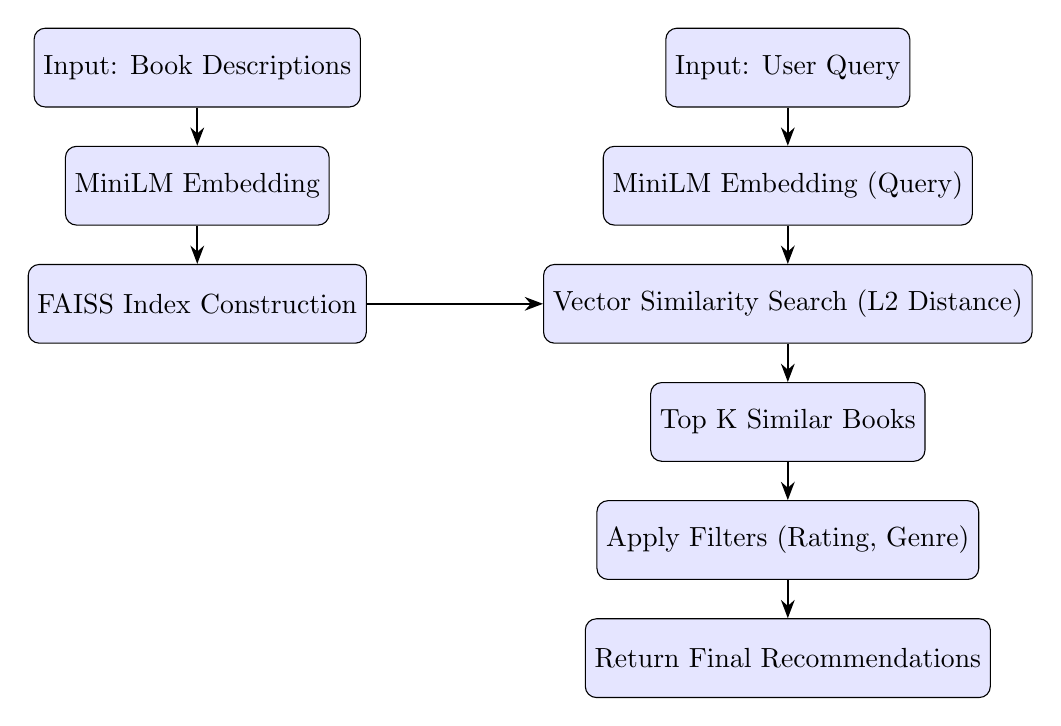
\begin{tikzpicture}[node distance=1.5cm]

    \node (desc) [block] {Input: Book Descriptions};
    \node (minilm) [block, below of=desc] {MiniLM Embedding};
    \node (index) [block, below of=minilm] {FAISS Index Construction};
    
    \node (query) [block, right of=desc, xshift=6cm] {Input: User Query};
    \node (qembed) [block, below of=query] {MiniLM Embedding (Query)};
    \node (simsearch) [block, below of=qembed] {Vector Similarity Search (L2 Distance)};
    
    \node (topk) [block, below of=simsearch] {Top K Similar Books};
    \node (filter) [block, below of=topk] {Apply Filters (Rating, Genre)};
    \node (output) [block, below of=filter] {Return Final Recommendations};
    
    % Arrows
    \draw [arrow] (desc) -- (minilm);
    \draw [arrow] (minilm) -- (index);
    \draw [arrow] (query) -- (qembed);
    \draw [arrow] (qembed) -- (simsearch);
    \draw [arrow] (index) -- (simsearch);
    \draw [arrow] (simsearch) -- (topk);
    \draw [arrow] (topk) -- (filter);
    \draw [arrow] (filter) -- (output);
    
\end{tikzpicture}
\chapter{Dataset Exploration}
\label{chapter:dataset}

The project began with the public dataset by Castillo (2025), containing metadata for over 6,800 books. Initial inspection revealed missing or inconsistent fields such as authorship, categories, and descriptions. A modular preprocessing pipeline was built to clean, augment, and prepare the data for semantic modeling.

\section{Dataset Overview}
The original dataset (\texttt{books.csv}) included fields such as:
\begin{itemize}
\item \verb|isbn13|, \verb|title|, \verb|subtitle|, \verb|authors|
\item \verb|categories|, \verb|description|, \verb|published_year|
\item \verb|average_rating|, \verb|num_pages|
\end{itemize}
Key fields were combined and engineered into a unified \verb|full_title|, and several boolean \verb|has_*| flags were created for inspection and filtering.

\section{Data Cleaning and Augmentation}
Cleaning and augmentation were performed in multiple stages:
\begin{enumerate}
\item \textbf{Initial Checks:} Detected and logged missing or invalid entries.
\item \textbf{OpenLibrary Augmentation:} Filled in missing values such as \texttt{authors}, \texttt{num\_pages}, and \texttt{thumbnail}. Introduced \texttt{subjects}.
\item \textbf{Google Books API:} Prioritized short or missing descriptions and added alternate fields (e.g., \texttt{description\_google}).
\item \textbf{Field Comparison:} Logged mismatches in fields like title and author between sources. Created \texttt{alt\_*} fields where minor but significant discrepancies were found.
\item \textbf{Final Merging:} Consolidated \texttt{categories}, \texttt{subjects}, and \texttt{categories\_google} into a cleaned \texttt{final\_categories} field.
\end{enumerate}
Records with less than 9 words in the final description were removed, reducing the dataset from 6,810 to 6,572 entries.

\section{Feature Engineering}
New fields were engineered to support classification and filtering:
\begin{itemize}
\item \verb|words_in_description| \textemdash{} token count of description
\item \verb|description_length| \textemdash{} character count of enriched description
\item \verb|has_*| flags \textemdash{} completeness indicators for filtering
\end{itemize}
These were used both for data readiness assessments and visualization.

\section{Exploratory Analysis}
Visual and statistical analysis was used to inform thresholds and highlight data issues:
\begin{itemize}
\item \textbf{Missing Values:} \verb|openlib_values_heatmap.png|
\item \textbf{Rating Distribution:} \verb|rating_distribution.png|
\item \textbf{Publication Year:} \verb|publication_year_distribution.png|
\item \textbf{Category Frequency:} \verb|top_categories.png|
\item \textbf{Short Descriptions:} \verb|less_than_50_words_description.png|
\item \textbf{Metadata Conflicts:} \verb|reexp_mismatch_counts.png|
\end{itemize}
These figures helped guide filtering strategies and offered insight into metadata quality.

\section{Outcome}
After augmentation and filtering, 6,572 books remained. These were passed to the category inference pipeline (Chapter~\ref{chapter:category-inference}), where further refinement reduced the set to 5,160 high-confidence entries suitable for semantic embedding and indexing.
\chapter{Category Inference}
\label{chapter:categories}

To enable semantic filtering and genre-aware recommendations, each book was assigned one or more thematic categories. This process combined zero-shot classification, keyword-based fallback strategies, and confidence-based filtering.

\section{Zero-Shot Classification with BART-MNLI}
Each book's metadata was combined into an \texttt{augmented\_description}, containing title, author, publication year, and description. This composite text was passed into the \texttt{facebook/bart-large-mnli} model using Hugging Face’s zero-shot classification pipeline.

Thirteen candidate labels were defined (e.g., \textit{Fantasy}, \textit{Love}, \textit{Non-fiction}). For each label, a confidence score was returned. Only scores $\geq 0.4$ were retained to ensure relevance. Books often received multiple labels.

\section{Keyword-Based Fallback Enrichment}
For books with weak model predictions or no confident labels, a curated list of keywords was used to infer likely genres. These fallback rules were only triggered if the corresponding category was not already predicted.

For example:
\begin{itemize}
    \item \textbf{Fantasy:} \textit{wizard}, \textit{magic}, \textit{dragon}
    \item \textbf{Science Fiction:} \textit{cyborg}, \textit{space travel}, \textit{AI}
    \item \textbf{Love:} \textit{romance}, \textit{relationship}, \textit{passion}
\end{itemize}

Fallback tagging increased recall and thematic coverage. Out of 6,572 entries, 4,665 received at least one fallback label.

\section{Refinement and Category Merging}
To reduce noise and improve label interpretability, overlapping or ambiguous categories were merged:
\begin{itemize}
    \item \textit{Biography} + \textit{History} $\rightarrow$ \textit{Historical}
    \item \textit{Suspense} + \textit{Detective} $\rightarrow$ \textit{Mystery}
    \item \textit{Poetry} + \textit{Philosophy} $\rightarrow$ \textit{Philosophy \& Poetry}
\end{itemize}

\begin{figure}[H]
    \centering
    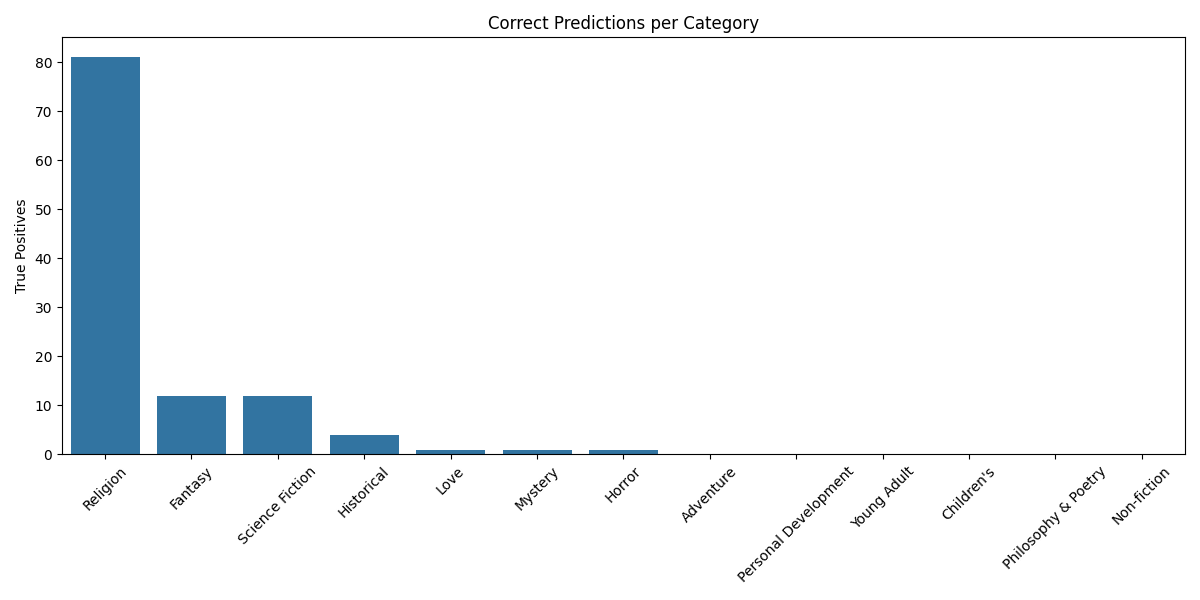
\includegraphics[width=0.9\textwidth]{figures/refine_category_prediction_matches.png}
    \caption{Prediction Matches per Category: Bar chart of true positives per category. Reflects model strength in domains like Fantasy and Love and highlights where fallback logic is critical.}
    \label{fig:refine_category_prediction_matches}
\end{figure}

Per-category precision, recall, and F1 scores were calculated by comparing predicted labels to a cleaned set of original tags. Figure~\ref{fig:refine_category_prediction_matches} shows prediction matches by category.

\section{Confidence Metrics and Filtering}
To prepare the dataset for embedding and indexing, multiple metrics were computed:
\begin{itemize}
    \item \texttt{max\_score} — Highest score among all predicted labels
    \item \texttt{filtered\_avg\_score} — Mean score of predictions $\geq 0.2$
    \item \texttt{score\_std} — Standard deviation across all label scores
    \item \texttt{num\_categories} — Count of confident labels retained
\end{itemize}

A row was retained if it met all of the following:
\begin{itemize}
    \item \texttt{description\_length} $\geq 200$ characters
    \item \texttt{filtered\_avg\_score} $\geq 0.2$
    \item \texttt{max\_score} $\geq 0.4$
    \item \texttt{num\_categories} $> 0$
\end{itemize}

This reduced the dataset from 6,572 to 5,160 high-confidence books.

\section{Length vs Confidence Correlation}
To verify that longer descriptions produce better classifications, correlation coefficients were computed:
\begin{itemize}
    \item Pearson $r = 0.398$, $p < 0.0001$
    \item Spearman $\rho = 0.261$, $p < 0.0001$
\end{itemize}

\begin{figure}[H]
    \centering
    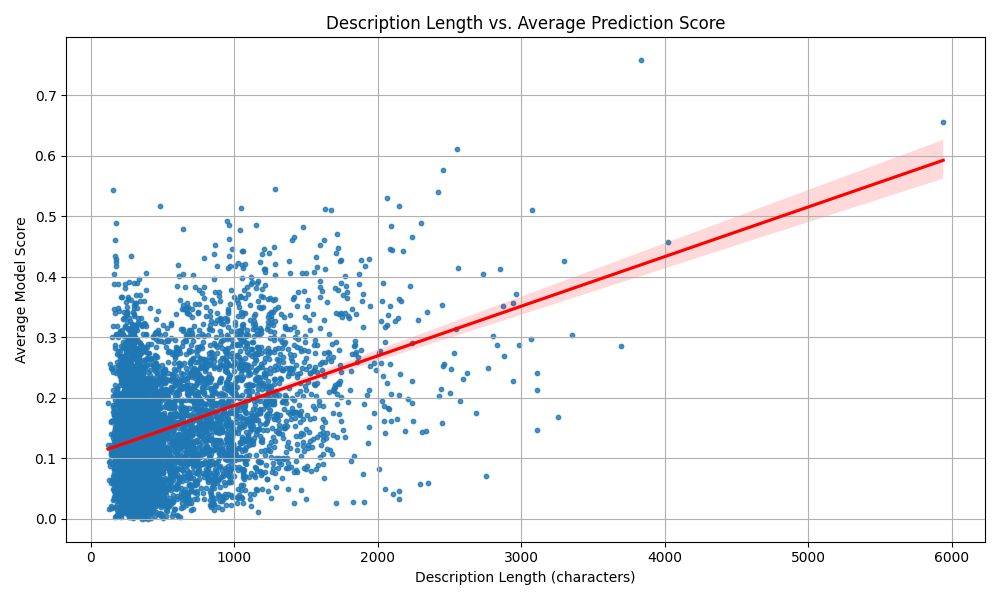
\includegraphics[width=0.9\textwidth]{figures/category_refined_description_length_vs_avg_score.png}
    \caption{Description Length vs. Confidence Score: A regression plot showing the positive correlation between description length and average model confidence.}
    \label{fig:category_refined_description_length_vs_avg_score}
\end{figure}

\begin{figure}[H]
    \centering
    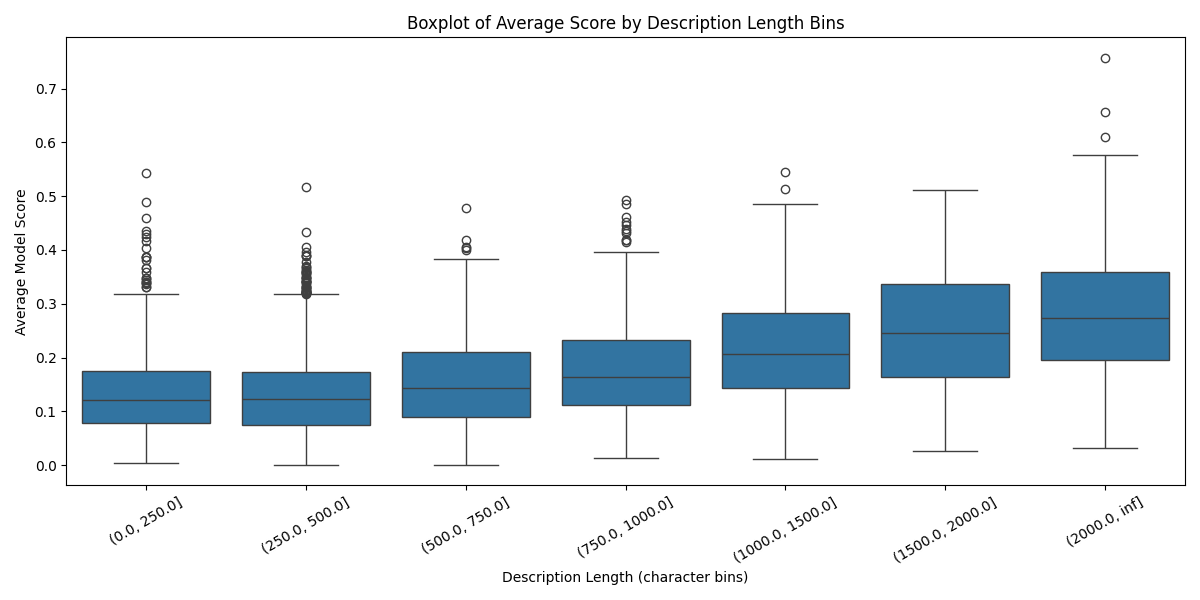
\includegraphics[width=0.9\textwidth]{figures/category_refined_avg_score_by_length_bin.png}
    \caption{Score by Length Bin: A boxplot displaying score variation across binned description lengths.}
    \label{fig:category_refined_avg_score_by_length_bin}
\end{figure}

These results indicate a moderate positive relationship. Figure~\ref{fig:category_refined_description_length_vs_avg_score} visualizes the regression, while Figure~\ref{fig:category_refined_avg_score_by_length_bin} shows variation across bins.

These findings supported a minimum \texttt{description\_length} of 200 characters during filtering.
\chapter{Text Embedding}
\label{chapter:embedding}

The core of the recommendation system lies in transforming books and queries into a shared semantic space. 
This is accomplished by generating sentence embeddings that encode the meaning of input text into numerical vectors. Once embedded, semantic similarity can be computed between queries and books.

\section{Sentence Embedding Theory}
\label{sec:embedding-theory}

Sentence embeddings are dense vector representations of variable-length text sequences. 
They enable comparison of textual content by mapping semantically similar sentences to nearby points in vector space. The process relies on transformer-based models.

Let $f(t)$ be the embedding function applied to a string $t$, producing a vector $\vec{v} \in \mathbb{R}^{384}$:
\begin{equation}
\vec{v} = f(t), \quad \vec{v} \in \mathbb{R}^{384}
\end{equation}

This project uses \texttt{all-MiniLM-L6-v2} from the Hugging Face \texttt{sentence-transformers} library, which produces 384-dimensional embeddings. 
It offers an excellent balance between speed and semantic quality, making it ideal for offline inference on CPU hardware.

\section{Embedding Implementation}
\label{sec:embedding-implementation}

Text embeddings were generated using a composite string field \texttt{search\_text}, constructed for each book as follows:

\begin{verbatim}
Title: {full_title}. Author: {authors}. Description: {description}
\end{verbatim}

This format ensures that both metadata and narrative content contribute to the semantic embedding. The following steps were performed:
\begin{enumerate}
    \item Loaded the final dataset \texttt{books\_indexed.csv}.
    \item Encoded each \texttt{search\_text} entry using MiniLM.
    \item Saved the resulting matrix of shape $(n, 384)$ to memory.
    \item Added all vectors to a FAISS index (see Chapter~\ref{chapter:faiss}).
    \item Saved metadata with vectors to \texttt{books\_indexed\_with\_embeddings.csv}.
\end{enumerate}

\section{Embedding Configuration}
\label{sec:embedding-config}

The embedding stage used the following parameters:
\begin{itemize}
    \item \textbf{Model:} \texttt{all-MiniLM-L6-v2}
    \item \textbf{Library:} \texttt{sentence-transformers}
    \item \textbf{Embedding Dimension:} 384
    \item \textbf{Distance Metric:} L2 (Euclidean)
    \item \textbf{Backend:} CPU inference
    \item \textbf{Input Field:} \texttt{search\_text}
    \item \textbf{Entries Embedded:} 5,160 books
\end{itemize}

\section{Summary}
\label{sec:embedding-summary}

The embedding pipeline enabled semantic similarity computations between books and queries. Using a compact transformer model, each entry was encoded into a vector capturing its latent meaning. 
This allowed content-based querying without relying on metadata fields like genre, author popularity, or user behavior. The resulting vectors were stored in a FAISS index for efficient similarity search.

\chapter{Vector Similarity Search with FAISS}
\label{chapter:faiss}

Once books and queries are embedded into the same semantic space, the system must identify the most relevant books for a given user input. This is achieved using vector similarity search. In this project, the FAISS (Facebook AI Similarity Search) library is used to enable fast and accurate nearest-neighbor retrieval over the 5,160 book vectors.

\section{Similarity Search Theory}
\label{sec:similarity-theory}

Let \( \vec{q} \in \mathbb{R}^{384} \) represent the embedded user query, and let \( \{\vec{b}_1, \vec{b}_2, \dots, \vec{b}_n\} \) denote the embedded book vectors. The similarity between the query and each book is computed using squared L2 (Euclidean) distance:

\begin{equation}
    \text{dist}(\vec{q}, \vec{b}_i) = \|\vec{q} - \vec{b}_i\|_2^2
\end{equation}

The top \( k \) nearest neighbors (i.e., those with the smallest distances) are returned as recommended books. This approach assumes that semantically similar texts lie close together in vector space.

\section{Why FAISS?}
\label{sec:faiss-choice}

FAISS is optimized for fast similarity search over high-dimensional vectors. It was selected for this project because it:

\begin{itemize}
    \item \textbf{Performs well on CPU} — fast enough for real-time use
    \item \textbf{Supports exact and approximate search} — adaptable for scale
    \item \textbf{Offers simple integration with NumPy and PyTorch}
    \item \textbf{Runs offline} — no internet connection required
\end{itemize}

This implementation uses \texttt{IndexFlatL2}, a brute-force index that performs exact nearest-neighbor search using squared L2 distance. It is suitable for small to medium datasets and does not require tuning.

\section{Implementation}
\label{sec:similarity-implementation}

After the embeddings were generated (see Chapter~\ref{chapter:embedding}), the similarity search process was implemented as follows:

\begin{enumerate}
    \item Initialize a \texttt{faiss.IndexFlatL2} index with vector dimension 384.
    \item Add the 5,160 book vectors to the index.
    \item At runtime:
    \begin{itemize}
        \item Embed the user query using the same MiniLM model.
        \item Use FAISS to find the top \( k \) nearest book vectors.
        \item Retrieve metadata from \texttt{books\_indexed\_with\_embeddings.csv}.
    \end{itemize}
\end{enumerate}

The system achieves sub-second response times on consumer-grade laptops using only CPU.

\section{Summary}
\label{sec:similarity-summary}

FAISS powers the core similarity engine of the recommender system. Combined with MiniLM embeddings, it enables local, real-time, and semantically aware recommendations. The entire matching process relies solely on content, requiring no user profiles or interaction history.

\chapter{User Interface}
\label{chapter:interface}

The user interface enables interaction with the semantic book recommendation system. 
While not a machine learning component, it plays a crucial role in usability, filtering, and presentation. 
The interface is implemented using \texttt{Streamlit}, a lightweight Python framework suitable for local-first applications.

\section{Design Principles}
\label{sec:ui-design}

The UI was designed with simplicity and responsiveness in mind. It supports end-to-end offline operation. Design goals included:

\begin{itemize}
    \item Concept-based natural language search
    \item Multi-faceted filtering by category and rating
    \item Minimal dependencies and fast startup
    \item Clear presentation of recommendations
\end{itemize}

All inference and retrieval logic runs locally.

\section{Query Workflow}
\label{sec:ui-query-workflow}

The system accepts a free-form text query from the user (e.g., \textit{``Books about surviving on Mars''}). The workflow proceeds as follows:

\begin{enumerate}
    \item Query is embedded using the MiniLM model.
    \item The FAISS index returns the top 60 nearest book vectors.
    \item Filtering and sorting options are applied.
    \item Six book cards are rendered per page.
\end{enumerate}

This approach allows expressive, language-based search.

\section{Filtering and Sorting}
\label{sec:ui-filtering}

Users can refine results with:

\begin{itemize}
    \item \textbf{Category filter:} Multi-select widget for genre labels
    \item \textbf{Rating sort:} Toggle for ascending/descending order
    \item \textbf{Pagination:} Adjustable page selection for navigation
\end{itemize}

Filters are applied after FAISS similarity search.

\section{Result Display}
\label{sec:ui-display}

Each result is rendered as a card containing:

\begin{itemize}
    \item Book cover image (URL with fallback)
    \item Full title and author
    \item Average rating, number of pages, and publication year
    \item Description excerpt (up to 300 characters)
    \item Refined categories
\end{itemize}

The layout ensures readability and intuitive navigation.

\section{Privacy and Offline Execution}
\label{sec:ui-privacy}

The application is designed for full offline use:

\begin{itemize}
    \item No tracking, cookies, or login
    \item No data transmission to external servers
    \item Book data, models, and index are stored locally
\end{itemize}

This ensures data privacy, fast load times, and compatibility with low-resource environments.

\section{Summary}
\label{sec:ui-summary}

The Streamlit interface allows users to interact with the system seamlessly. 
Natural language search, combined with real-time filtering and semantic recommendations, creates an intuitive and private discovery experience.
\chapter{Performance and Evaluation Challenges}
\label{chapter:performance}

This chapter outlines how the system’s performance was evaluated, given the absence of user feedback and labeled test data. Traditional metrics such as accuracy or precision are not directly applicable to semantic similarity tasks without ground truth. Therefore, evaluation is divided into subjective, statistical, and system-level components.

\section{Evaluation Without Labels}
\label{sec:no-labels}

The system does not predict a fixed label or class. Instead, it embeds both queries and books in a shared vector space and retrieves nearest neighbors using semantic distance. As a result:

\begin{itemize}
    \item There is no single “correct” recommendation per query.
    \item Precision/recall-based metrics cannot be used reliably.
    \item Feedback mechanisms like click-through or engagement data are unavailable in an offline setting.
\end{itemize}

This necessitates alternative evaluation strategies.

\section{Qualitative Evaluation}
\label{sec:qualitative-eval}

Evaluation relied on exploratory queries and manual inspection of results. Test queries covered a range of genres, tones, and abstraction levels. Examples include:

\begin{itemize}
    \item ``Existential loneliness in space''
    \item ``Post-apocalyptic survival story''
    \item ``Books that explore grief through fantasy''
\end{itemize}

Results were judged based on alignment between the query and the content of the returned book descriptions. This human-in-the-loop approach confirmed that semantically aligned results were typically returned.

\section{Category Inference Evaluation}
\label{sec:category-eval}

Although the original dataset lacked consistent genre labels, the quality of inferred categories was assessed via:

\begin{itemize}
    \item Retaining classification confidence scores per label
    \item Filtering by a threshold of 0.4 (see Chapter~\ref{chapter:categories})
    \item Computing precision, recall, and F1 scores for a subset of trusted entries
    \item Visualizing match counts and fallback coverage
\end{itemize}

Certain categories (e.g., \textit{Fantasy}, \textit{Love}) were strongly predicted by the model, while others (e.g., \textit{Philosophy \& Poetry}) relied more heavily on fallback keyword enrichment.

\section{Responsiveness and Latency}
\label{sec:latency}

Performance was measured on a consumer-grade laptop (no GPU):

\begin{itemize}
    \item Query embedding time (MiniLM): $< 0.2$ seconds
    \item FAISS top-60 vector search: $< 10$ ms
    \item Streamlit UI rendering (6 cards per page): $< 2$ seconds including image fallback
\end{itemize}

This confirms that the system operates in real time on modest hardware, supporting its offline-first goal.

\section{Scalability Considerations}
\label{sec:scaling}

While the current dataset (5,160 entries) is manageable, scaling raises practical challenges:

\begin{itemize}
    \item \textbf{Indexing:} FAISS IndexFlatL2 is efficient but linear in search time; approximate methods (e.g., HNSW) may be needed for larger corpora.
    \item \textbf{Re-embedding:} Changing models or descriptions requires recomputing all embeddings.
    \item \textbf{Filtering:} UI-side filtering and sorting scale linearly with post-search result volume.
\end{itemize}

Future extensions should consider vector compression, batch processing, and caching.

\section{Limitations of Offline Evaluation}
\label{sec:limitations}

Offline evaluation limits the types of insights that can be gathered:

\begin{itemize}
    \item \textbf{Relevance:} Relies solely on developer judgment
    \item \textbf{Discovery:} Cannot measure novelty or serendipity
    \item \textbf{Bias Detection:} Overrepresentation of certain authors or genres may go unnoticed
\end{itemize}

These are acceptable trade-offs in the context of a local, user-respecting prototype.

\section{Summary}
\label{sec:performance-summary}

Evaluation focused on semantic quality, practical responsiveness, and offline usability. Despite the lack of supervised benchmarks, confidence filtering, manual validation, and runtime measurements demonstrated that the system is performant and aligned with its design goals.

\chapter{Conclusion}
\label{chapter:conclusion}

This chapter summarizes the findings and outcomes of the project, reflects on its limitations, and revisits the original research questions.

\section{Discussion}
\label{sec:discussion}

This project demonstrated that transformer-based models can power a local, content-only book recommendation system. Without requiring user profiles or collaborative filtering, the system delivers semantically meaningful recommendations based entirely on book metadata and free-text queries.

The end-to-end system consisted of:
\begin{itemize}
    \item Augmented and cleaned metadata for over 6,800 books
    \item Zero-shot genre inference using BART-MNLI with fallback keyword enrichment
    \item Semantic embeddings via MiniLM
    \item FAISS-based vector search
    \item A responsive, private UI implemented in Streamlit
\end{itemize}

With no reliance on internet access, the system runs entirely offline and respects user privacy. It is suitable for low-resource environments and educational use cases.

\section{Conclusion}
\label{sec:conclusion}

The system successfully addressed all four research sub-questions:

\begin{enumerate}
    \item \textbf{What techniques exist for embedding text into meaningful vectors?}  
    Pretrained sentence transformers like MiniLM encode text into high-dimensional semantic vectors, enabling rich similarity comparisons.

    \item \textbf{How can vector similarity be used for finding similar books?}  
    FAISS enables fast nearest-neighbor retrieval in vector space, allowing queries to return top-matching books based on content alone.

    \item \textbf{How can genre categories be inferred and used for filtering?}  
    BART-MNLI enables zero-shot classification of genre labels. Fallback keyword rules and confidence filtering improve label coverage and reliability.

    \item \textbf{What are the limitations of a local, content-only recommender?}  
    The system lacks personalization and behavior-driven refinement. However, it compensates with transparency, offline execution, and semantic precision.
\end{enumerate}

\noindent
\textbf{Main research question:}

\begin{quote}
\textit{How can a local ML model be used to recommend books based on natural language descriptions, relying only on locally running models?}
\end{quote}

This was answered by developing and validating a fully local recommendation system that performs semantic classification, embedding, indexing, and retrieval — all on-device.

\section{Reflection}
\label{sec:reflection}

The project offered valuable insights into building ML-powered applications under strict resource constraints. Key lessons include:

\begin{itemize}
    \item \textbf{Description quality drives results:} Well-written descriptions significantly enhance semantic accuracy.
    \item \textbf{Fallbacks expand coverage:} Keyword-based strategies improve classification when the model lacks confidence.
    \item \textbf{Local-first ML is viable:} Even compact transformer models provide robust performance on consumer hardware.
    \item \textbf{Simplicity over complexity:} Lightweight, modular design reduced failure points and increased maintainability.
\end{itemize}

With more time, the system could be extended to include:

\begin{itemize}
    \item Comparison of embedding models (e.g., MPNet, SBERT)
    \item Re-ranking of results based on metadata
    \item Interactive user feedback or offline learning
\end{itemize}

The project demonstrates that privacy-respecting, offline-first NLP systems are not only possible but practical. This aligns with emerging interest in edge-based AI and user-sovereign computing.
In a forward-looking perspective, the system could serve as a foundation for more complex applications - such as personalized learning assistants or local knowledge bases - 
further enhancing the utility of AI in everyday life while respecting user privacy.


%% Prevent urls running into margins in bibliography
\setcounter{biburlnumpenalty}{7000}
\setcounter{biburllcpenalty}{7000}
\setcounter{biburlucpenalty}{7000}

%% Add bibliography
\printbibliography[heading=bibintoc,title={References}]

%% ----------------------------------------------------------------------
%%    Appendix (Letters for chapters)
%% ----------------------------------------------------------------------

\appendix

% Glossaries
\chapter{Glossary of Terms}
\label{appendix:glossary}

This appendix defines key terms used throughout the project, with a focus on Machine Learning, Natural Language Processing, and Information Retrieval. Each entry aims to explain the term in accessible language, suitable for readers with a general computer science background.

\begin{description}
    \item[AI (Artificial Intelligence):] The simulation of human intelligence in machines that can reason, learn, and make decisions.
    \item[Attention Mechanism:] A component of neural networks, especially transformers, that allows the model to focus on relevant parts of the input sequence when making predictions.
    \item[Augmentation (Data):] The process of enriching data with external sources to fill in missing values or increase its descriptive quality.
    \item[BART (Bidirectional and Auto-Regressive Transformer):] A transformer model used for text generation and classification tasks. In this project, it powers zero-shot classification.
    \item[BERT (Bidirectional Encoder Representations from Transformers):] A transformer-based model that generates contextual embeddings for text, capturing semantic meaning. It is foundational for many NLP tasks.
    \item[Category Inference:] Assigning thematic or genre labels to text entries based on their content.
    \item[Classification:] The task of assigning predefined labels to text based on its content. In this project, it is used to infer book genres.
    \item[Cold Start Problem:] A challenge in recommender systems where there is insufficient data about new users or items to make accurate recommendations.
    \item[Content-Based Recommendation:] A technique that recommends items based on their attributes rather than user behavior.
    \item[Cosine Similarity:] A metric that measures the cosine of the angle between two vectors, indicating how similar they are in direction regardless of magnitude.
    \item[Dimensionality Reduction:] Techniques used to reduce the number of features in data while preserving important information, often used before similarity search.
    \item[Embedding:] The transformation of text into a numeric vector that captures its meaning in a high-dimensional space.
    \item[Embedding Function:] A function or model that converts text into a vector representation. In this project, it is implemented using MiniLM.
    \item[Embedding Model:] A neural network that transforms text into fixed-length numeric vectors, capturing semantic meaning. This project uses MiniLM for sentence embeddings.
    \item[Embedding-Based Search:] A search technique that uses vector representations of text to find semantically similar items rather than relying solely on keyword matching.
    \item[FAISS (Facebook AI Similarity Search):] A library that enables efficient vector similarity search, often used for large-scale nearest neighbor search.
    \item[FAISS Index:] A data structure used by FAISS to store and retrieve high-dimensional vectors efficiently. It allows for fast similarity searches.
    \item[Feature Extraction:] The process of transforming raw data into a set of features that can be used for machine learning tasks.
    \item[Filtering:] Reducing a set of results based on certain constraints (e.g., rating threshold, genre tag).
    \item[Fine-Tuning:] The process of taking a pre-trained model and training it further on a specific dataset to adapt it to a particular task.
    \item[GloVe (Global Vectors for Word Representation):] A model that generates word embeddings by analyzing word co-occurrence statistics in a corpus, capturing global semantic relationships.
    \item[Ground Truth:] The actual, real-world values or labels used as a benchmark to evaluate model predictions.
    \item[Hybrid Recommendation:] A system that combines multiple recommendation strategies, such as content-based and collaborative filtering, to improve results.
    \item[Inference (Model):] The process of using a trained model to make predictions on new, unseen data.
    \item[L2 Distance (Euclidean):] A metric that measures the straight-line distance between two vectors in space.
    \item[Local-First Design:] A system architecture that prioritizes local computation and storage, minimizing reliance on external servers.
    \item[MiniLM:] A lightweight sentence embedding model that provides efficient semantic representations with low computational cost.
    \item[MultiNLI (Multi-Genre Natural Language Inference):] A dataset used for training models on natural language inference tasks, where the goal is to determine if a hypothesis logically follows from a premise.
    \item[Natural Language Generation (NLG):] A subfield of NLP that focuses on generating human-like text from structured data or other inputs.
    \item[Natural Language Inference (NLI):] A task in NLP where the goal is to determine if a hypothesis logically follows from a premise, often used for zero-shot classification.
    \item[Natural Language Processing (NLP):] A field of AI focused on the interaction between computers and human language, enabling machines to understand, interpret, and generate text.
    \item[Natural Language Understanding (NLU):] A subfield of NLP that focuses on enabling machines to understand the meaning and intent behind human language.
    \item[Overfitting:] When a model learns the training data too well, including its noise, resulting in poor generalization to new data.
    \item[Pearson Correlation:] A measure of the linear correlation between two variables, indicating how well one can predict the other.
    \item[Pre-trained Model:] A model that has been previously trained on a large dataset and can be fine-tuned for specific tasks, reducing the need for extensive training from scratch.
    \item[Precision (Information Retrieval):] The proportion of retrieved items that are actually relevant.
    \item[Query:] A user-inputted string used to search or retrieve information from a system.
    \item[Ranking:] The process of ordering items (e.g., search results or recommendations) based on their relevance or predicted interest to the user.
    \item[Recall (Information Retrieval):] The proportion of relevant items that are successfully retrieved by a search or recommendation system.
    \item[Recommender System:] A system that suggests items of interest to users based on various algorithms.
    \item[Semantic Search:] A search technique that considers the meaning of the query rather than just keyword matching.
    \item[Sentence Embedding:] A vector representation of a sentence that captures its semantic meaning.
    \item[Similarity Metric:] A function that quantifies how alike two objects (such as vectors or texts) are, commonly used in search and recommendation.
    \item[Spearman Correlation:] A non-parametric measure of rank correlation that assesses how well the relationship between two variables can be described by a monotonic function.
    \item[Stop Words:] Common words (such as "the", "is", "and") that are often removed during text preprocessing because they carry little semantic meaning.
    \item[Streamlit:] A lightweight Python framework for building interactive web interfaces for machine learning and data science applications.
    \item[Token:] A basic unit of text, such as a word or subword, that is processed by NLP models. Tokenization is the process of converting text into these units. 
    \item[Tokenization:] The process of breaking down text into smaller units (tokens), such as words or subwords, for further processing.
    \item[Transformer:] A neural network architecture designed to handle sequential data, commonly used in language models.
    \item[User Profile:] A representation of a user's preferences, interests, or behavior, used to personalize recommendations.
    \item[Vector Index:] A data structure that stores embedded vectors for fast similarity retrieval.
    \item[Word Embedding:] A representation of words in a continuous vector space, capturing semantic relationships. Examples include Word2Vec and GloVe.
    \item[Word2Vec:] A model that generates word embeddings by predicting surrounding words in a sentence, capturing semantic relationships based on context.
    \item[Zero-Shot Classification:] A method where a model assigns labels it has never seen during training, using semantic understanding.
\end{description}

\chapter{Symbol Dictionary}
\label{appendix:symbols}

This appendix summarizes the mathematical symbols used in the project. Each symbol is listed with its meaning and the context in which it appears.

\begin{description}
    \item[\( t \)] Input text or string to be embedded (e.g., book description or user query).

    \item[\( f(t) \)] Embedding function that maps a string to a high-dimensional vector using a pretrained model.

    \item[\( \vec{v} \)] The resulting vector embedding of the input text.

    \item[\( \mathbb{R}^{d} \)] The \(d\)-dimensional real-valued vector space in which embeddings are located. In this project, \( d = 384 \).

    \item[\( \vec{q} \)] The vector representation of a user query.

    \item[\( \vec{b}_i \)] The vector representation of the \(i\)-th book in the dataset.

    \item[\( \|\vec{q} - \vec{b}_i\|_2^2 \)] The squared L2 (Euclidean) distance between the query and a book vector, used for similarity ranking.

    \item[\( k \)] The number of top search results to retrieve based on vector similarity.

    \item[\( n \)] Total number of book entries in the vector index.

    \item[\( r \)] Pearson correlation coefficient, used to measure the linear relationship between description length and confidence.

    \item[\( \rho \)] Spearman rank correlation coefficient, used to evaluate monotonic relationships between two ranked variables.
\end{description}

\chapter{Figures}
\label{appendix:figures}

This appendix presents the figures generated throughout the data processing pipeline. Each figure is introduced in the order it was produced, along with a short explanation of what it represents and how it informed decisions in the pipeline.

\begin{figure}[H]
    \centering
    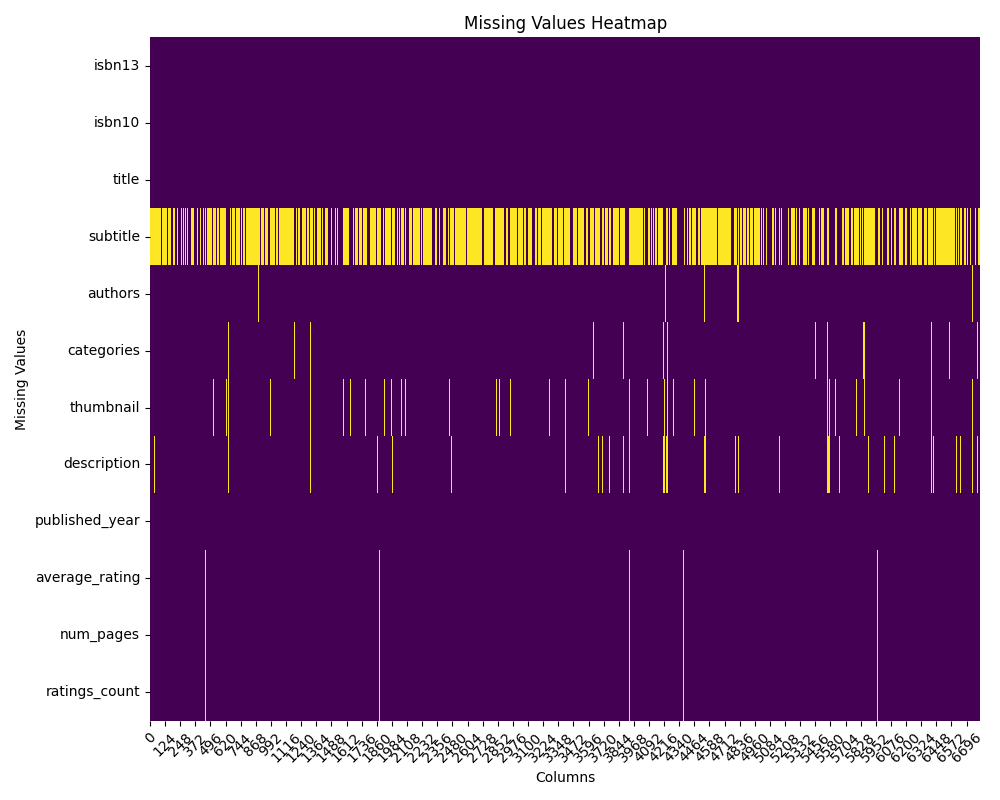
\includegraphics[width=0.9\textwidth]{figures/missing_values_heatmap.png}
    \caption{Missing Values Heatmap: Visualizes the density of missing fields in the original dataset. The heatmap highlights common gaps such as missing subtitles, authors, and thumbnails, prompting the need for augmentation.}
\end{figure}

\begin{figure}[H]
    \centering
    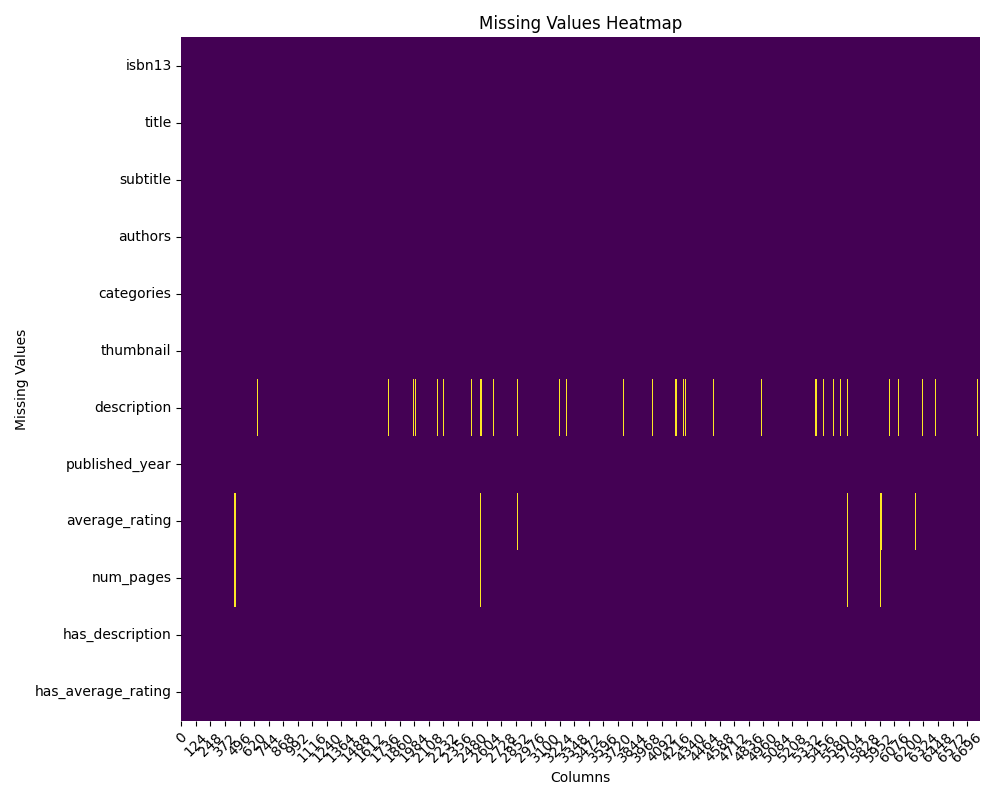
\includegraphics[width=0.9\textwidth]{figures/openlib_values_heatmap.png}
    \caption{OpenLibrary Completion Heatmap: Displays the remaining missing values after OpenLibrary augmentation. It shows improvements in coverage of fields like subtitles, page counts, and published years.}
\end{figure}

\begin{figure}[H]
    \centering
    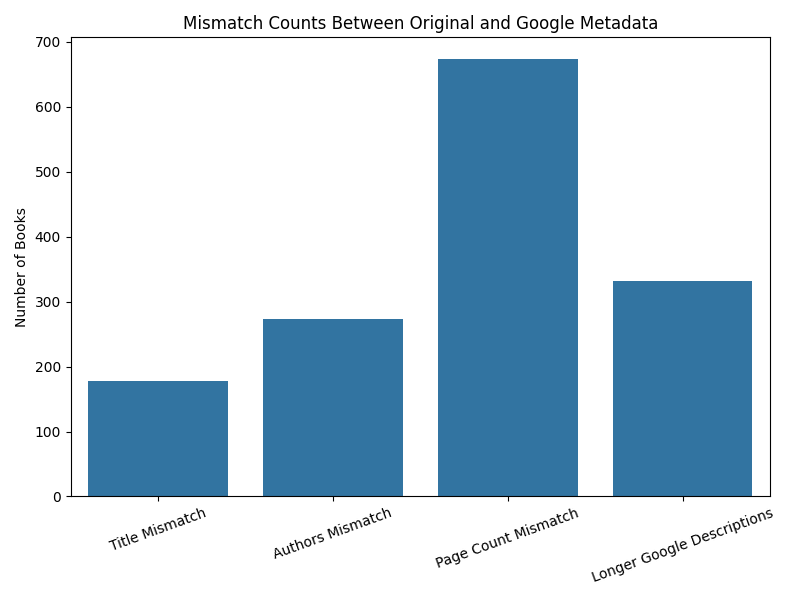
\includegraphics[width=0.9\textwidth]{figures/reexp_mismatch_counts.png}
    \caption{Metadata Conflict Counts: A bar chart showing the number of books with mismatches in title, author, or page count across sources. This justified creation of alternative metadata fields.}
\end{figure}

\begin{figure}[H]
    \centering
    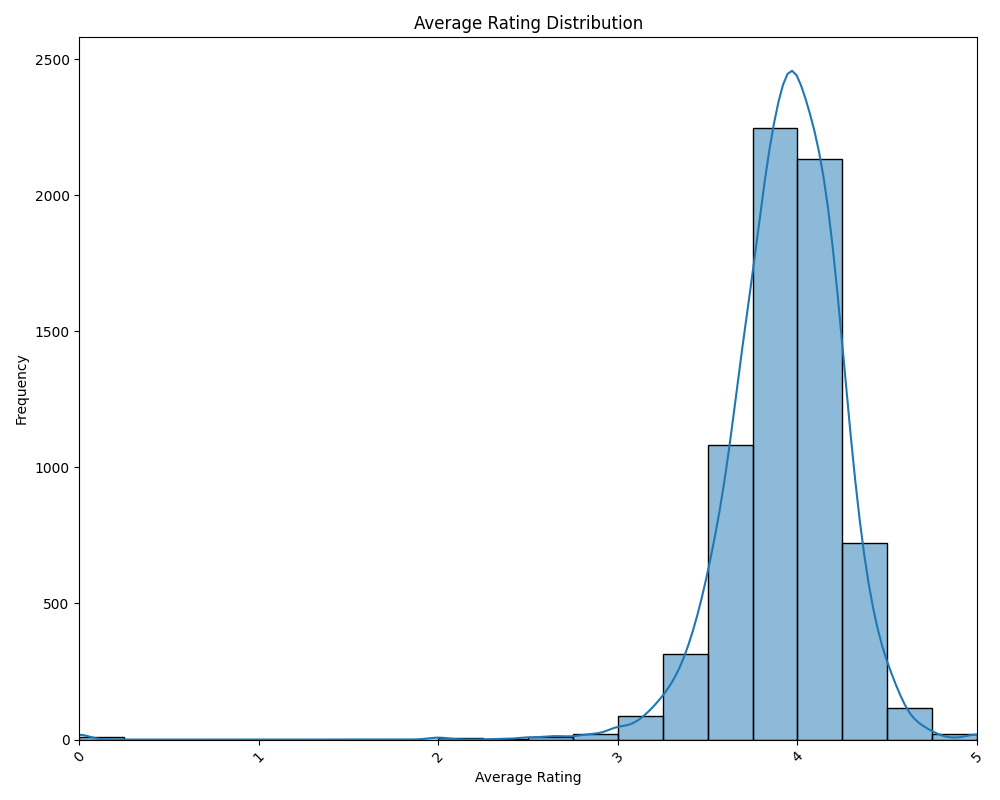
\includegraphics[width=0.9\textwidth]{figures/rating_distribution.png}
    \caption{Rating Distribution: Histogram of average book ratings. The skew toward higher ratings is typical for user-generated content and informed filter default settings.}
\end{figure}

\begin{figure}[H]
    \centering
    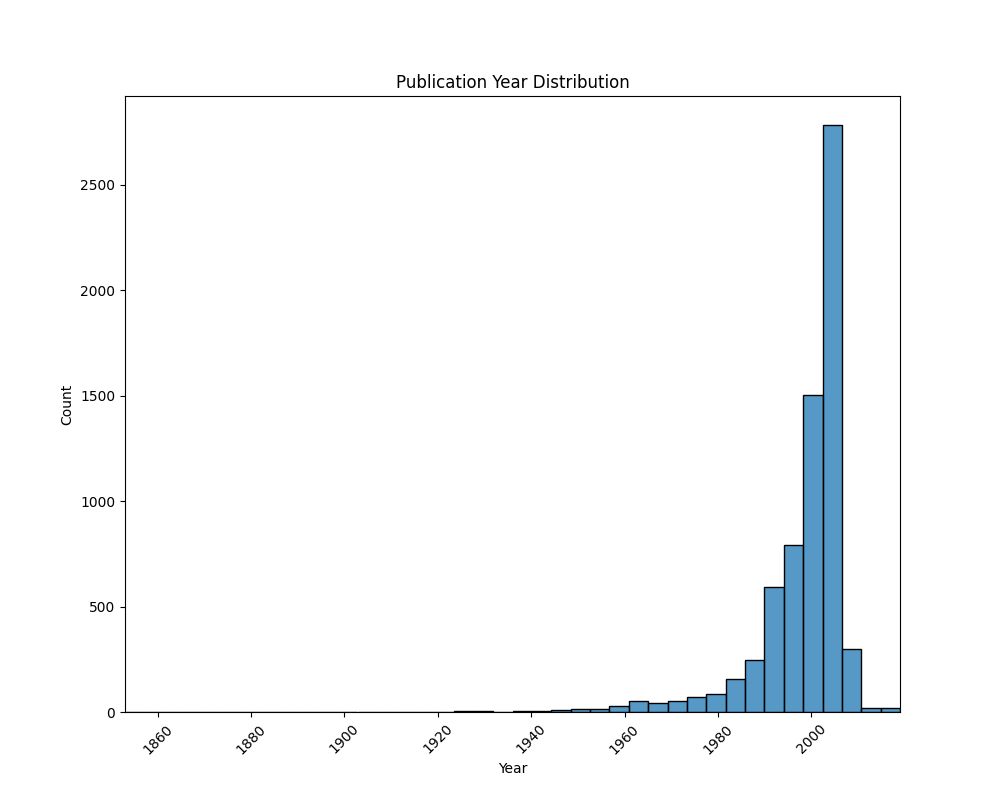
\includegraphics[width=0.9\textwidth]{figures/publication_year_distribution.png}
    \caption{Publication Year Distribution: Shows the number of books published per year. The majority are post-2000, indicating a recency bias that may impact topic coverage.}
\end{figure}

\begin{figure}[H]
    \centering
    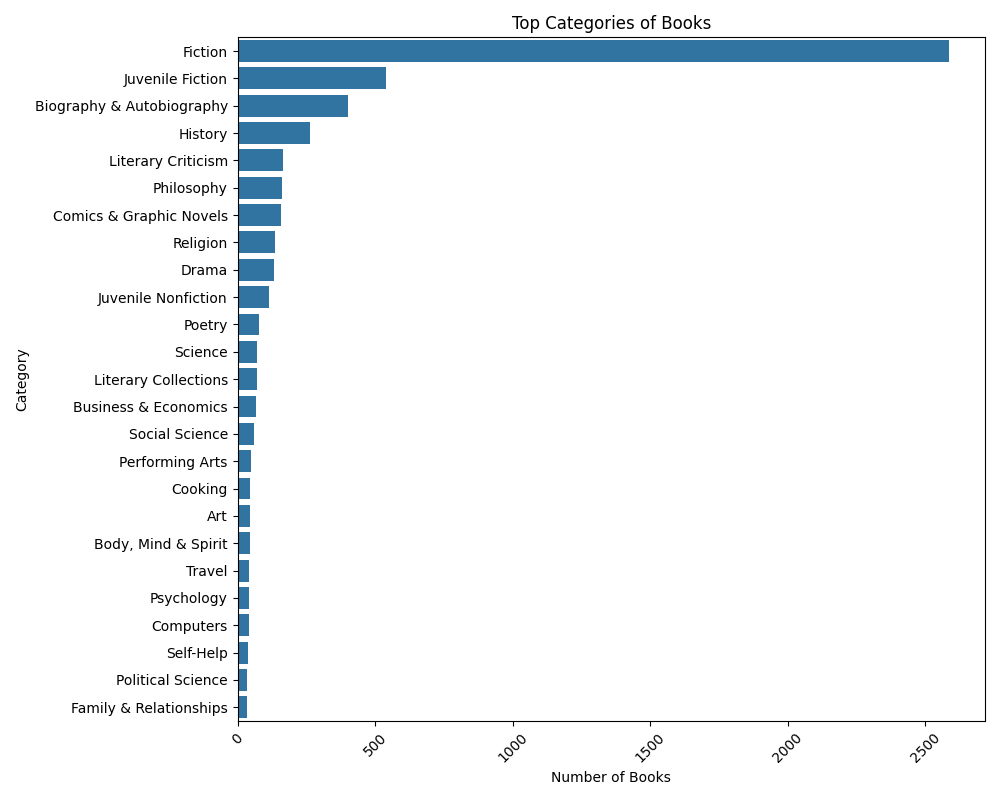
\includegraphics[width=0.9\textwidth]{figures/top_categories.png}
    \caption{Top Categories: A bar chart of the most frequent category labels in the original dataset. This informed the definition of candidate labels for zero-shot classification.}
\end{figure}

\begin{figure}[H]
    \centering
    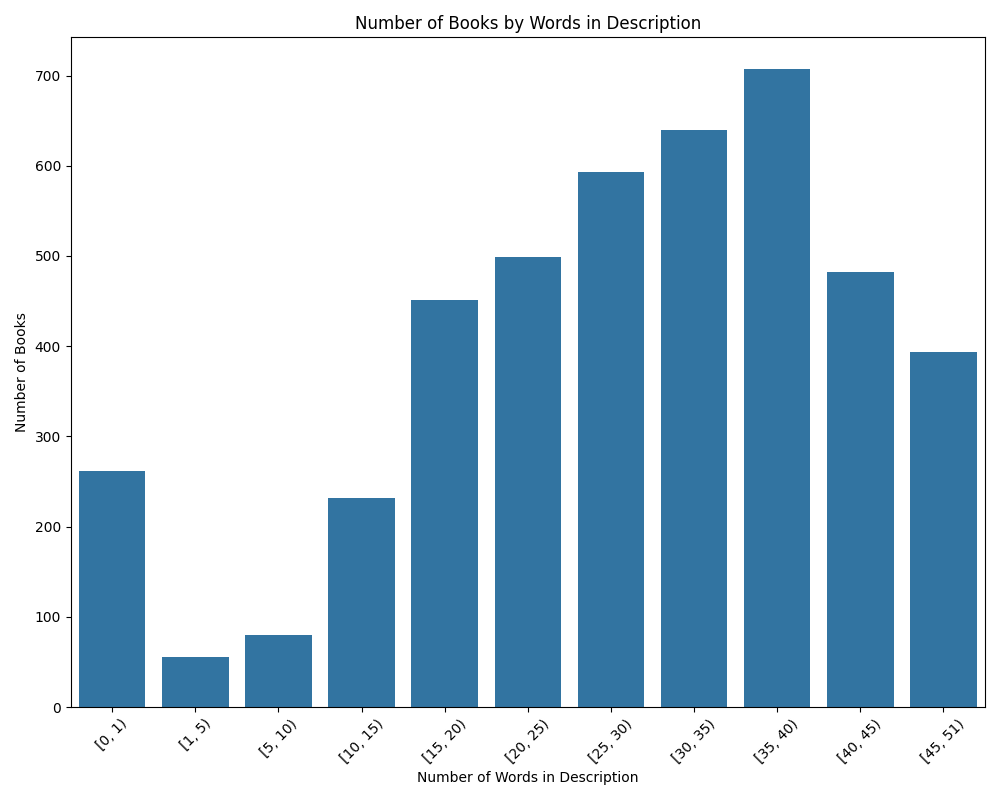
\includegraphics[width=0.9\textwidth]{figures/less_than_50_words_description.png}
    \caption{Books with Short Descriptions: Distribution of books with fewer than 50 words in their descriptions. These entries were flagged for enrichment or removal.}
\end{figure}

\begin{figure}[H]
    \centering
    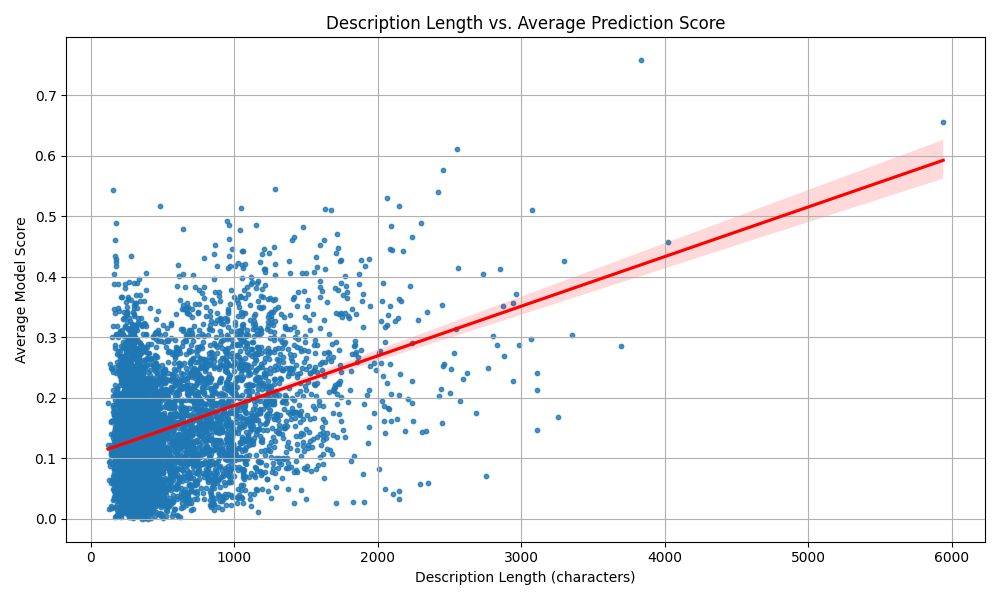
\includegraphics[width=0.9\textwidth]{figures/category_refined_description_length_vs_avg_score.png}
    \caption{Description Length vs. Confidence Score: A regression plot showing the positive correlation between description length and average model confidence. This supported the threshold of 200 characters.}
\end{figure}

\begin{figure}[H]
    \centering
    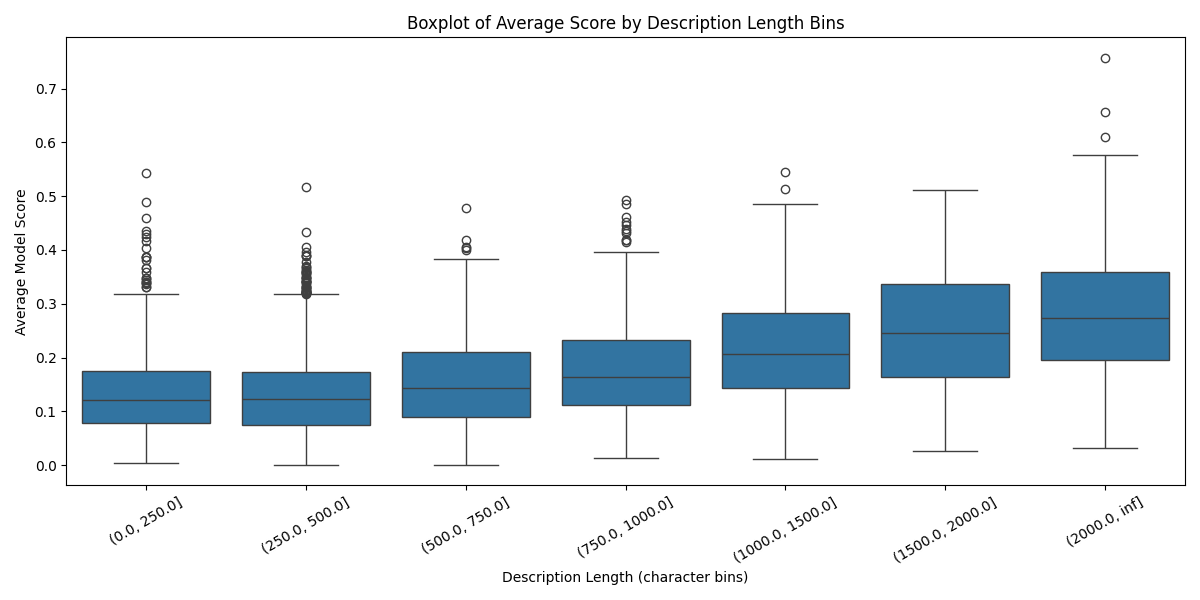
\includegraphics[width=0.9\textwidth]{figures/category_refined_avg_score_by_length_bin.png}
    \caption{Score by Length Bin: A boxplot displaying score variation across binned description lengths. Helps visualize consistency and reliability of model outputs by text richness.}
\end{figure}

\begin{figure}[H]
    \centering
    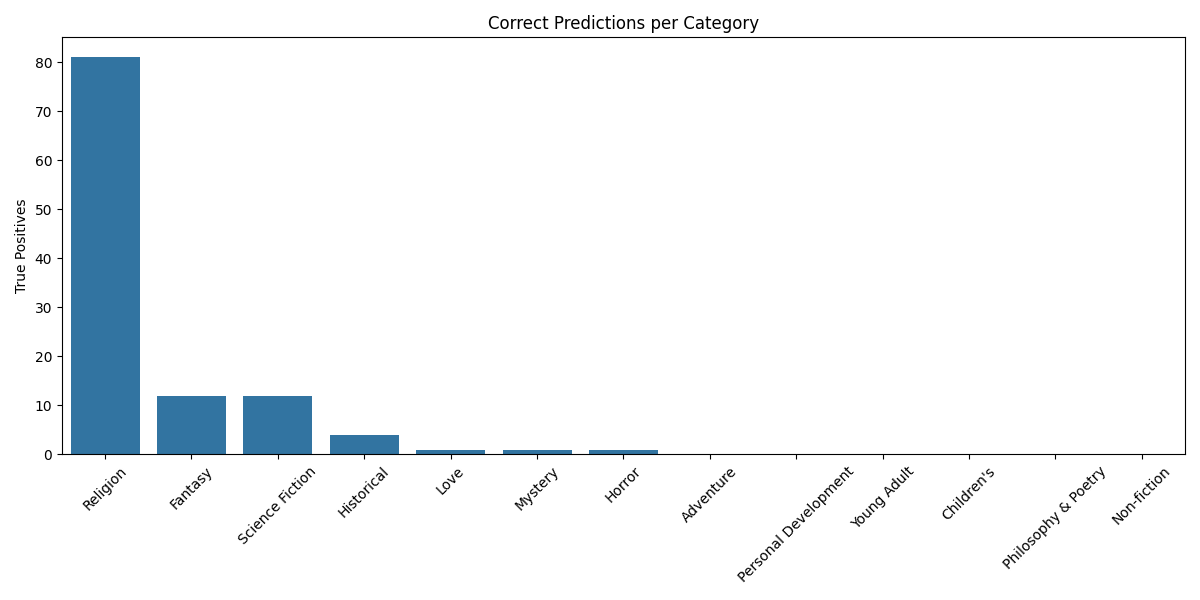
\includegraphics[width=0.9\textwidth]{figures/refine_category_prediction_matches.png}
    \caption{Prediction Matches per Category: Bar chart of true positives per category. Reflects model strength in domains like Fantasy and Love and highlights where fallback logic is critical.}
\end{figure}

% Theoretical Appendices
\chapter{Theory of Sentence Embeddings}
\label{appendix:embedding-theory}

This appendix expands on the theoretical and practical foundations of sentence embeddings. These representations serve as the basis for semantic similarity throughout the system, as discussed in Chapter~\ref{chapter:embedding}. Understanding how they are constructed and used is essential for grasping the logic behind embedding-based search and classification.

\section{From Words to Vectors}
In traditional NLP, words are first tokenized and represented numerically. Early methods like one-hot encoding fail to capture semantic relationships between words. This motivated the development of distributed representations — where words are embedded in continuous vector spaces.

Word embeddings like Word2Vec~\parencite{mikolov2013efficient} and GloVe~\parencite{pennington2014glove} map words with similar contexts to nearby points in a high-dimensional space. However, they produce static embeddings: the word "bank" will have the same vector whether referring to a financial institution or a riverbank.

\section{Sentence Embeddings}
Sentence embeddings aim to extend this idea to whole sentences or paragraphs. They encode variable-length text into fixed-length dense vectors that capture meaning, context, and structure.

Formally, let:
\[
f(t) = \vec{v}, \quad \vec{v} \in \mathbb{R}^d
\]
where \( t \) is the input sentence, \( f \) is an embedding function (typically a neural model), and \( d \) is the dimensionality of the embedding space.

\section{Transformer-Based Embeddings}
Transformer models~\parencite{vaswani2017attention} have become the backbone of modern NLP. Instead of relying on fixed context windows, they use self-attention to consider the entire sentence when encoding each word.

Sentence-BERT (SBERT)~\parencite{reimers2019sentencebert} fine-tunes transformer architectures to generate sentence-level embeddings. This project uses the distilled variant \texttt{all-MiniLM-L6-v2}, which balances semantic performance with CPU efficiency.

\subsection*{Architecture Overview}
Below is a simplified diagram of the embedding process using a transformer:

\begin{figure}[H]
\centering
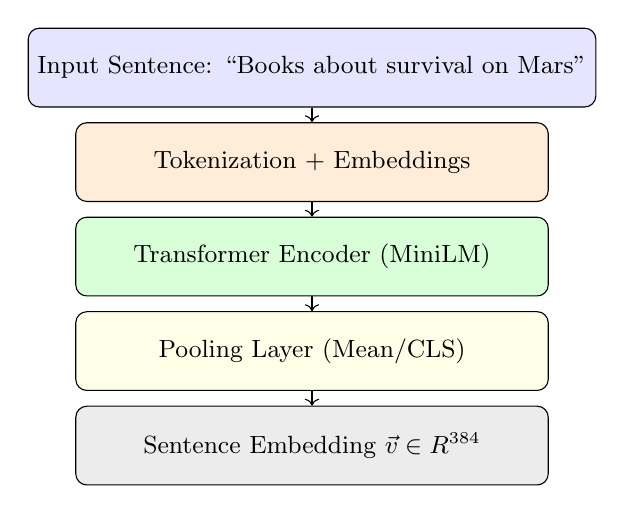
\begin{tikzpicture}[node distance=1.2cm, every node/.style={font=\small}]
    \node (input) [draw, rounded corners, minimum width=6cm, minimum height=1cm, fill=blue!10] {Input Sentence: ``Books about survival on Mars''};

    \node (tokens) [below of=input, draw, rounded corners, minimum width=6cm, minimum height=1cm, fill=orange!15] {Tokenization + Embeddings};

    \node (transformer) [below of=tokens, draw, rounded corners, minimum width=6cm, minimum height=1cm, fill=green!15] {Transformer Encoder (MiniLM)};

    \node (pooling) [below of=transformer, draw, rounded corners, minimum width=6cm, minimum height=1cm, fill=yellow!10] {Pooling Layer (Mean/CLS)};

    \node (vector) [below of=pooling, draw, rounded corners, minimum width=6cm, minimum height=1cm, fill=gray!15] {Sentence Embedding \( \vec{v} \in \mathbb{R}^{384} \)};

    \draw[->] (input) -- (tokens);
    \draw[->] (tokens) -- (transformer);
    \draw[->] (transformer) -- (pooling);
    \draw[->] (pooling) -- (vector);
\end{tikzpicture}
\caption{Pipeline for generating a sentence embedding}
\end{figure}

\section{Similarity Measures}
Once embedded, sentences can be compared using vector similarity. Common measures include:

\begin{itemize}
    \item \textbf{Cosine similarity:} 
    \[
    \cos(\theta) = \frac{\vec{v}_1 \cdot \vec{v}_2}{\|\vec{v}_1\| \|\vec{v}_2\|}
    \]
    Measures the angle between two vectors, emphasizing direction over magnitude.

    \item \textbf{Euclidean (L2) distance:}
    \[
    \|\vec{v}_1 - \vec{v}_2\|_2^2
    \]
    Measures straight-line distance. This project uses L2 distance for compatibility with FAISS.
\end{itemize}

\section{Intuitive Example}
Consider these two sentences:

\begin{quote}
\emph{``A man is walking a dog.''} \\
\emph{``Someone strolls through the park with a pet.''}
\end{quote}

Despite having no identical words, their embeddings lie close together in semantic space, enabling meaningful comparisons beyond keyword overlap.

\section{Limitations and Challenges}
While powerful, sentence embeddings have limitations:

\begin{itemize}
    \item Cannot perfectly disambiguate sarcasm, irony, or negation
    \item Performance degrades on domain-specific jargon
    \item Quality depends heavily on description clarity and length
\end{itemize}

\section{Conclusion}
Sentence embeddings are a foundational tool for semantic search and classification. By transforming language into geometry, they unlock flexible, content-aware systems that work without user histories or explicit labels.

Models like MiniLM make such capabilities available even on modest hardware — aligning with the project's offline-first design.


\chapter{Vector Similarity and Search}
\label{appendix:similarity-theory}

This appendix elaborates on the mathematical foundations and implementation considerations behind vector similarity search — the mechanism used to match queries and books in semantic space.

\section{Motivation}
Traditional search engines rely on exact term overlap. However, semantically similar phrases often differ lexically:

\begin{quote}
\textit{``Books about exploring loneliness in space''} vs. \textit{``Isolation in science fiction''}
\end{quote}

Embedding-based systems overcome this limitation by projecting both queries and documents into a shared vector space. The task then becomes: \textit{find the vectors nearest to a query vector}.

\section{Mathematical Background}
Let \( \vec{q} \in \mathbb{R}^d \) represent a query embedding, and let \( \{ \vec{b}_1, \vec{b}_2, \dots, \vec{b}_n \} \subset \mathbb{R}^d \) be the embeddings of all books.

The most similar books are found by minimizing the distance function:
\[
\text{dist}(\vec{q}, \vec{b}_i) = \|\vec{q} - \vec{b}_i\|_2^2
\]

Alternatively, cosine similarity can be used:
\[
\cos(\theta) = \frac{\vec{q} \cdot \vec{b}_i}{\|\vec{q}\| \|\vec{b}_i\|}
\]

In this system, squared Euclidean (L2) distance is used to match the FAISS index type.

\section{Geometric Intuition}
In geometric terms, the embedding space is like a multi-dimensional landscape. Each book occupies a fixed location. A query becomes a “probe,” and similarity search identifies the closest “peaks.”

\begin{figure}[H]
\centering
\begin{tikzpicture}[scale=1.2]
    % Axes
    \draw[->] (-2, 0) -- (4, 0) node[right] {\( x_1 \)};
    \draw[->] (0, -1.5) -- (0, 3) node[above] {\( x_2 \)};
    
    % Query vector
    \draw[->, thick, red] (0, 0) -- (1.2, 1.8) node[above right] {\( \vec{q} \)};
    
    % Book vectors
    \draw[->, thick, blue] (0, 0) -- (2, 2.1) node[above] {\( \vec{b}_1 \)};
    \draw[->, thick, blue] (0, 0) -- (1.5, 1.2) node[below right] {\( \vec{b}_2 \)};
    \draw[->, thick, blue] (0, 0) -- (3, -0.5) node[below] {\( \vec{b}_3 \)};
    
    % Arc showing angle
    \draw[dashed] (0.9, 1.35) arc[start angle=56, end angle=75, radius=1cm];
    \node at (1.15, 1.1) {\( \theta \)};
\end{tikzpicture}
\caption{Visualizing semantic proximity between query and book vectors}
\end{figure}

The smaller the angle or distance, the more semantically relevant the book is.

\section{Indexing with FAISS}
FAISS~\parencite{johnson2019billion} is an open-source library from Facebook AI that enables efficient similarity search over high-dimensional vectors.

This project uses:
- \texttt{IndexFlatL2} — brute-force, exact L2 search
- CPU-only backend for offline execution
- Sub-second retrieval of top-\( k \) results from over 5,000 book vectors

For large datasets, approximate indices (e.g., HNSW, IVF) can be substituted for faster but slightly less precise searches.

\section{Advantages of Vector Search}
\begin{itemize}
    \item \textbf{Language-aware:} Finds relevant matches even with low lexical overlap
    \item \textbf{Scalable:} Compatible with millions of documents with indexing
    \item \textbf{Offline-capable:} Entire process runs locally without cloud dependencies
\end{itemize}

\section{Limitations}
\begin{itemize}
    \item \textbf{Semantic ambiguity:} Vector proximity does not guarantee relevance in all cases
    \item \textbf{Cold start:} Requires embeddings for all documents up front
    \item \textbf{Interpretability:} Search decisions are hard to explain due to vector abstraction
\end{itemize}

\section{Conclusion}
Vector similarity search replaces keyword matching with a geometric proximity task in semantic space. Combined with embedding models, this enables robust content-based recommendations even in resource-constrained, offline environments.

\chapter{Theory of Zero-Shot Classification}
\label{appendix:zsc-theory}

This appendix elaborates on zero-shot classification (ZSC), which is used in this system to infer thematic categories for books. Unlike traditional classification methods, ZSC does not require labeled training data for each class. Instead, it relies on a language model’s ability to understand and reason about class labels as natural language.

\section{What is Zero-Shot Classification?}
Traditional classification models require supervised training data — examples of each class to learn from. Zero-shot classification removes this constraint. A model trained on natural language inference (NLI) is reused for classification by rephrasing the task as a premise–hypothesis pair.

\begin{quote}
\textbf{Premise:} “This book is about elves and ancient magic.” \\
\textbf{Hypothesis:} “This text is about fantasy.”
\end{quote}

The model estimates the probability that the hypothesis is entailed by the premise. If high, the label (“fantasy”) is considered appropriate.

\section{Model Foundations}
This project uses \texttt{facebook/bart-large-mnli}, a transformer model fine-tuned on the MultiNLI corpus~\parencite{williams2018broad}. The model performs classification by computing entailment scores between the input and each label reformulated as a natural sentence.

\subsection*{Architecture Overview}
\begin{figure}[H]
\centering
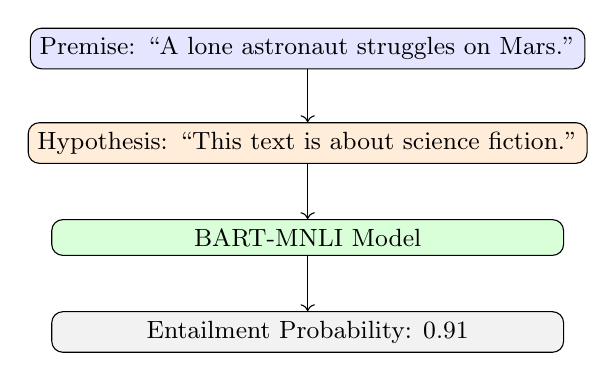
\begin{tikzpicture}[node distance=1.2cm, every node/.style={font=\small}]
    \node (premise) [draw, fill=blue!10, minimum width=6.5cm, rounded corners] {Premise: “A lone astronaut struggles on Mars.”};
    \node (hypo) [below of=premise, draw, fill=orange!15, minimum width=6.5cm, rounded corners] {Hypothesis: “This text is about science fiction.”};
    \node (model) [below of=hypo, draw, fill=green!15, minimum width=6.5cm, rounded corners] {BART-MNLI Model};
    \node (output) [below of=model, draw, fill=gray!10, minimum width=6.5cm, rounded corners] {Entailment Probability: 0.91};

    \draw[->] (premise) -- (hypo);
    \draw[->] (hypo) -- (model);
    \draw[->] (model) -- (output);
\end{tikzpicture}
\caption{Zero-shot classification via textual entailment}
\end{figure}

\section{How It Works in Practice}
Given a book description and a list of candidate genres (e.g., “fantasy”, “science fiction”, “romance”), each label is evaluated independently as a hypothesis. Labels with high entailment scores are retained.

This approach enables:
\begin{itemize}
    \item Multi-label classification: multiple genres can apply
    \item Dynamic label sets: new genres can be introduced without retraining
    \item Minimal supervision: no need for annotated datasets
\end{itemize}

\section{Confidence Thresholding}
The model returns a confidence score for each label. Labels below a threshold (e.g., 0.4) are discarded to reduce noise. Labels just below the threshold may be added through fallback keyword rules.

\section{Fallback Strategies}
To improve coverage when ZSC fails, a rule-based system checks for genre-specific keywords in the description or title. This hybrid approach balances model generalization with deterministic recall.

\section{Limitations}
\begin{itemize}
    \item \textbf{Surface sensitivity:} ZSC may be confused by subtle phrasing
    \item \textbf{High compute cost:} Each label requires a full model pass
    \item \textbf{Bias leakage:} Pretrained models may carry genre biases
\end{itemize}

\section{Conclusion}
Zero-shot classification enables genre inference without labeled examples, making it ideal for low-resource, flexible systems. By treating labels as hypotheses, it leverages the general reasoning ability of transformer models — aligning well with the offline and adaptable design goals of this project.

\chapter{Data Cleaning and Augmentation}
\label{appendix:data-cleaning}

This appendix explores the techniques used for cleaning and augmenting book metadata, which was essential for building a semantically rich, searchable dataset. It addresses how inconsistencies, missing values, and weak textual descriptions were handled to support effective downstream ML tasks.

\section{Why Data Quality Matters}
In embedding-based systems, input quality directly affects output relevance. Ambiguous or sparse descriptions produce poor embeddings, reducing semantic precision. Similarly, inconsistent or missing metadata can weaken classification and filtering performance.

\section{Cleaning Pipeline Overview}
The dataset originally included over 7,000 book records, aggregated from various sources with variable completeness. The following steps were applied:

\begin{enumerate}
    \item Dropped entries missing title or description
    \item Removed duplicates and outliers (e.g., unusually long texts)
    \item Normalized text casing and whitespace
    \item Replaced null fields with placeholders or estimations
    \item Removed boilerplate text (e.g., “No description available”)
\end{enumerate}

\subsection*{Cleaning Heuristics}
These heuristics were used to streamline cleaning:
\begin{itemize}
    \item Length thresholds (e.g., min 100 characters for description)
    \item Filtering based on punctuation density (flagging auto-generated entries)
    \item Removing descriptions composed entirely of keywords or tags
\end{itemize}

\section{Data Augmentation}
To improve the semantic richness of inputs, the following augmentation methods were used:

\subsection*{(1) Composite Description Field}
A new field \texttt{search\_text} was created by merging:

\begin{verbatim}
Title: {title}. Author: {authors}. Description: {description}
\end{verbatim}

This gave more context to the embedding model, emphasizing title and author relevance.

\subsection*{(2) External Source Integration}
Descriptions were extended where possible using public APIs:

\begin{itemize}
    \item Open Library API
    \item Google Books API
\end{itemize}

If a book had a matching identifier (e.g., ISBN), missing fields like description, page count, or rating were filled in.

\subsection*{(3) Metadata Derivation}
Additional fields were derived:
\begin{itemize}
    \item \textbf{Book age:} computed from publication year
    \item \textbf{Page count bins:} converted to categorical buckets
    \item \textbf{Rating level:} numerical rating mapped to qualitative tiers
\end{itemize}

\section{Correlation Checks}
Correlation analysis between description length and classification confidence was conducted to justify filtering. Spearman’s \( \rho \) and Pearson’s \( r \) were computed and visualized to support design decisions (see Appendix~\ref{appendix:figures}).

\section{Fallback Design Philosophy}
Where automatic tools failed (e.g., ZSC output too sparse), manual logic was introduced:
\begin{itemize}
    \item Keyword-based genre tagging (e.g., “spaceship” → Sci-Fi)
    \item Heuristic label propagation within author clusters
\end{itemize}

This hybrid design emphasizes robustness over purity — especially valuable for offline and low-resource contexts.

\section{Limitations and Trade-offs}
\begin{itemize}
    \item Augmentation may introduce minor inconsistencies (e.g., mismatched genres across sources)
    \item Some fields were inferred from partial matches and are best-effort estimates
    \item Reliance on third-party APIs, while limited, introduces variation in format and tone
\end{itemize}

\section{Conclusion}
Data preparation is foundational to the success of semantic systems. The cleaning and augmentation pipeline ensured that even lightweight models received rich, structured inputs — enabling effective classification and retrieval downstream.

\chapter{Local-First System Design Principles}
\label{appendix:local-first}

This appendix outlines the principles behind local-first architecture, as applied to this project’s end-to-end recommendation system. It explains how privacy, autonomy, and offline usability influenced the choice of tools and methods.

\section{What is Local-First Software?}
Local-first software prioritizes performing all computation and storage on the user’s own device. Network access is optional, not essential. Key motivations include:

\begin{itemize}
    \item \textbf{Privacy:} No personal data is sent to remote servers.
    \item \textbf{Reliability:} The system functions without internet access.
    \item \textbf{Ownership:} The user retains full control over their data and execution.
\end{itemize}

This paradigm aligns well with AI applications where model inference is possible without cloud dependencies.

\section{Application to This Project}
Every step of the pipeline was designed to run locally:

\begin{itemize}
    \item \textbf{Model inference:} All embedding and classification done using CPU-friendly models (MiniLM, BART-MNLI).
    \item \textbf{Storage:} All data and embeddings stored in local CSV and FAISS index files.
    \item \textbf{Interface:} The Streamlit app runs entirely within a browser on localhost.
\end{itemize}

\section{Architectural Choices}
The system was built around modular, loosely coupled components:

\begin{enumerate}
    \item Python scripts for data ingestion, augmentation, and embedding
    \item FAISS index for efficient vector search
    \item Streamlit frontend for interaction
\end{enumerate}

Each step can be re-run or updated independently, supporting rapid experimentation and debugging.

\section{Trade-Offs and Limitations}
\begin{itemize}
    \item \textbf{No personalization:} Without user tracking or history, recommendations are purely content-based.
    \item \textbf{Compute constraints:} Model size is limited by local CPU/RAM availability.
    \item \textbf{No online learning:} The system does not evolve based on user behavior unless manually re-trained.
\end{itemize}

These limitations are acceptable within the project’s scope and enable greater user autonomy.

\section{Offline AI: Why It Matters}
Running AI locally is increasingly viable due to efficient models and improved hardware. Benefits include:

\begin{itemize}
    \item Resilience in low-connectivity environments (e.g., education, fieldwork)
    \item Cost reduction (no cloud inference or hosting fees)
    \item Alignment with GDPR and user-rights perspectives
\end{itemize}

\section{Comparison with Cloud-Based Systems}
{\small
\begin{tabular}{@{}p{4.5cm} p{4.5cm} p{4.5cm}@{}}
\toprule
\textbf{Aspect} & \textbf{Local-First} & \textbf{Cloud-Based} \\
\midrule
Latency & Sub-second (no network delay) & Depends on API round-trips \\
Privacy & No data leaves device & Data often logged/transferred \\
Scalability & Limited to local hardware & Scales elastically with demand \\
Update Mechanism & Manual or scripted & Centralized and automatic \\
Dependency & Self-contained & Relies on service availability \\
\bottomrule
\end{tabular}
}

\section{Conclusion}
Local-first design makes AI more accessible, ethical, and sustainable. By avoiding network reliance, the system empowers users to explore semantic search capabilities on their own terms, without compromising performance or flexibility.


\chapter{Evaluation and Performance Metrics}
\label{appendix:evaluation}

This appendix describes the evaluation strategy used to assess the performance of the local book recommendation system. Since no ground-truth labels or user feedback data were available, traditional supervised metrics (e.g., accuracy, precision, recall) could not be applied. Instead, alternative metrics were used to evaluate semantic relevance, system responsiveness, and overall usability.

\section{Constraints on Evaluation}
\begin{itemize}
    \item \textbf{No user history:} No personalized or collaborative filtering baseline.
    \item \textbf{No labeled test set:} No “correct” genre or match annotations.
    \item \textbf{Offline-only:} All testing conducted without server-side analytics or live monitoring.
\end{itemize}

This necessitated a human-in-the-loop, qualitative approach.

\section{Evaluation Criteria}
Four core criteria guided system evaluation:

\subsection*{1. Semantic Relevance}
Assessed whether the top-\( k \) results for a query were semantically aligned with its intent. This was evaluated manually using test queries such as:

\begin{quote}
\textit{“Books about surviving in space”} → Check that returned books involve space travel, isolation, or survival themes.
\end{quote}

In most test cases, at least 4 of the top 6 results were contextually appropriate.

\subsection*{2. Filtering Utility}
Tested whether genre and rating filters improved or restricted result precision. Filters were toggled and queries rerun to compare:

\begin{itemize}
    \item Breadth of result diversity
    \item Preservation of relevance post-filter
\end{itemize}

This highlighted that over-filtering may remove semantically correct results.

\subsection*{3. Responsiveness}
Measured latency of key operations on CPU-only hardware:

\begin{itemize}
    \item Query embedding: ~150ms
    \item FAISS search (top 60): <50ms
    \item Filtering and rendering: <300ms
\end{itemize}

Sub-second feedback ensured smooth interactivity.

\subsection*{4. Offline Functionality}
Validated that all components (embedding, classification, filtering, UI) function without network access. This included running:

\begin{itemize}
    \item Zero-shot classification with cached local models
    \item Full semantic search using only local vector index
    \item No calls to online services or third-party APIs
\end{itemize}

\section{Example Query Types}
Different categories of queries were tested:
\begin{itemize}
    \item \textbf{Thematic:} “Books about AI ethics”
    \item \textbf{Mood-driven:} “Something dark and mysterious”
    \item \textbf{Specific:} “Books like Dune”
\end{itemize}

Semantic embedding enabled flexible and expressive querying even when keywords were absent.

\section{Limitations of Evaluation}
\begin{itemize}
    \item No user feedback loop to refine metrics or iterate design
    \item No A/B testing against alternatives (e.g., TF-IDF or keyword search)
    \item Evaluation is largely anecdotal and lacks quantitative validation
\end{itemize}

Nevertheless, the qualitative results were consistent and satisfactory for the project scope.

\section{Conclusion}
Evaluation in low-data, offline-first ML projects requires adapted criteria. By focusing on semantic quality, system speed, and functional constraints, meaningful insights were still obtained. 
The framework can be extended in future work with automated tests or user trials.


%\chapter{Similarity Search with FAISS}
\label{appendix:faiss}

Similarity search is the task of finding items most similar to a given query in a high-dimensional vector space. This project uses FAISS (Facebook AI Similarity Search) to perform fast, exact nearest-neighbor lookups over book embeddings.

\section*{Motivation}
Books and queries are embedded into the same semantic vector space. To recommend relevant books, the system retrieves the closest vectors (books) to a given query vector.

\section*{What is FAISS?}
FAISS is a C++/Python library developed by Meta for fast search across large collections of dense vectors. It supports both exact and approximate search methods.

\section*{Indexing Method Used}
This system uses the exact search index:
\begin{itemize}
  \item \texttt{IndexFlatL2} — Computes L2 (Euclidean) distance between the query and all book vectors
  \item Suitable for small to medium datasets (\textasciitilde5,000 vectors)
  \item No compression or quantization
\end{itemize}

\section*{Search Workflow}
\begin{enumerate}
  \item Book metadata is converted to \texttt{search\_text} and embedded
  \item Vectors are added to a FAISS index
  \item At query time, the user input is embedded
  \item FAISS returns top-$k$ nearest neighbors
  \item Metadata is retrieved from the indexed CSV
\end{enumerate}

\section*{Distance Metric}
FAISS computes squared L2 distance:
\[ \text{dist}(\vec{q}, \vec{b}_i) = \| \vec{q} - \vec{b}_i \|_2^2 \]

Lower values indicate higher semantic similarity.

\section*{Benefits}
\begin{itemize}
  \item Extremely fast for exact matching on CPU
  \item Integrates easily with NumPy and PyTorch
  \item Fully offline and open source
\end{itemize}

\section*{Alternatives}
For larger datasets, approximate methods like HNSW, IVF, or PQ (quantization) may be more scalable but require tuning.

FAISS was ideal for this project due to its simplicity and performance at the given scale.
%\chapter{Confidence Filtering}
\label{appendix:confidence-filtering}

Confidence filtering is the process of retaining only high-certainty predictions from a model. In this project, it is used to ensure that category labels assigned to books are reliable.

\section*{Motivation}
Zero-shot classification produces a confidence score for each category. However, not all scores are meaningful — low-confidence predictions can lead to noisy or irrelevant labels.

\section*{Metrics Used}
Three metrics were computed for each book's classification output:

\begin{itemize}
  \item \textbf{max\_score} — the highest confidence score among all categories
  \item \textbf{filtered\_avg\_score} — average confidence score for predictions above a threshold (e.g., 0.2)
  \item \textbf{score\_std} — standard deviation of all confidence scores
\end{itemize}

\section*{Filtering Strategy}
To retain high-quality entries for indexing and UI use, books were required to meet all of the following:

\begin{itemize}
  \item \texttt{description\_length} $\geq$ 200 characters
  \item \texttt{filtered\_avg\_score} $\geq$ 0.2
  \item \texttt{max\_score} $\geq$ 0.4
  \item At least one predicted category
\end{itemize}

\section*{Why Multiple Metrics?}
\begin{itemize}
  \item \textbf{max\_score} ensures at least one strong category signal
  \item \textbf{filtered\_avg\_score} avoids noisy averages dominated by low scores
  \item \textbf{score\_std} (analyzed but not thresholded) helps detect ambiguous predictions
\end{itemize}

\section*{Impact}
These thresholds reduced the dataset from 6,572 to 5,160 entries, each with well-supported category labels and semantically rich descriptions. This filtering greatly improved the quality of recommendations.

Confidence filtering balances recall and precision, ensuring that the final indexed dataset is useful and trustworthy.

%\chapter{Fallback Classification with Keywords}
\label{appendix:keyword-fallback}

While zero-shot classification captured many semantic categories with high accuracy, some descriptions were too vague or short for the model to assign reliable labels. To compensate, a fallback strategy based on keyword matching was added.

\section*{Motivation}
Some books lack rich descriptions or use metaphoric language. For example, a horror book might avoid directly mentioning "ghosts" or "monsters" but still belong to the genre. Keywords help catch these implicit themes.

\section*{Keyword Lists}
Each predefined category was associated with a curated list of terms. For instance:
\begin{itemize}
  \item \textbf{Fantasy:} \texttt{magic, wizard, dragon, elf, spell}
  \item \textbf{Science Fiction:} \texttt{space, alien, robot, galaxy, dystopia}
  \item \textbf{Love:} \texttt{romance, passion, heartbreak, relationship}
\end{itemize}

These lists were handcrafted and refined iteratively during testing.

\section*{Matching Logic}
After zero-shot prediction:
\begin{itemize}
  \item Each description (or augmented description) was lowercased.
  \item Keyword presence was checked using regular expressions.
  \item Fallback labels were added only if not already predicted by the model.
\end{itemize}

\section*{Benefits}
\begin{itemize}
  \item Increases coverage of categories
  \item Captures under-expressed themes in sparse descriptions
  \item Keeps control in hands of the developer (interpretable logic)
\end{itemize}

\section*{Drawbacks}
\begin{itemize}
  \item Sensitive to phrasing and vocabulary
  \item May overfit to genre stereotypes (e.g., “dragon” always implies Fantasy)
  \item Requires manual tuning and maintenance
\end{itemize}

Fallback classification ensures that every book receives at least one thematic label, improving both UI filter functionality and downstream semantic search quality.

%\include{appendix/i-semantic-vs-keyword}

\end{document}